\documentclass[gmd, manuscript]{copernicus}

\begin{document}

\linenumbers

\title{Using Reactive Transport Codes to Provide Mechanistic Biogeochemistry
Representations in Global Land Surface Models}


\Author[1]{Guoping}{Tang}
\Author[1]{Fengming}{Yuan}
\Author[1,2]{Gautam}{Bisht}
\Author[3,4]{Glenn E.}{Hammond}
\Author[5]{Peter C.}{Lichtner}
\Author[1]{Jitendra}{ Kumar}
\Author[6]{Richard T.}{Mills}
\Author[1,7]{Xiaofeng}{Xu}
\Author[2,8]{Ben}{Andre}
\Author[1]{Forrest M.}{Hoffman}
\Author[1]{Scott L.}{Painter}
\Author[1]{Peter E.}{Thornton}

\affil[1]{Oak Ridge National Laboratory, Oak Ridge, Tennessee, United States}
\affil[2]{Lawrence Berkeley National Laboratory, Berkeley, California, United States}
\affil[3]{Pacific Northwest National Laboratory, Richland, Washington, United States}
\affil[4]{Sandia National Laboratories, Albuquerque, New Mexico, United States}
\affil[5]{OFM Research--Southwest, Santa Fe, New Mexico, United States}
\affil[6]{Intel Corporation, Hillsboro, Oregon, United States}
\affil[7]{San Diego State University, San Diego, California, United States}
\affil[8]{National Center for Atmospheric Research, Boulder, Colorado, United States}

\runningtitle{CLM-PFLOTRAN Biogeochemistry}

\runningauthor{Tang et al. 2015}

\correspondence{Peter E. Thornton (thorntonpe@ornl.gov), Scott L. Painter (paintersl@ornl.gov)}

\received{}
\pubdiscuss{} %% only important for two-stage journals
\revised{}
\accepted{}
\published{}

%% These dates will be inserted by Copernicus Publications during the typesetting process.

\firstpage{1}

\maketitle

This manuscript has been authored by UT-Battelle, LLC under Contract No.
DE-AC05-00OR22725 with the U.S. Department of Energy.  The United States
Government retains and the publisher, by accepting the article for publication,
acknowledges that the United States Government retains a non-exclusive,
paid-up, irrevocable, world-wide license to publish or reproduce the published
form of this manuscript, or allow others to do so, for United States Government
purposes.  The Department of Energy will provide public access to these results
of federally sponsored research in accordance with the DOE Public Access
Plan(http://energy.gov/downloads/doe-public-access-plan).


\clearpage
\begin{abstract}
We explore coupling to a configurable subsurface reactive transport
code as a flexible and extensible approach to biogeochemistry in land
surface models, to facilitate testing of alternative models and incorporation of
new understanding. A reaction network with the CLM-CN decomposition, nitrification,
denitrification, and plant uptake is used as an example. We implement the
reactions in the open-source PFLOTRAN code, coupled to the Community Land Model
(CLM), and test at Arctic, temperate, and tropical sites. To make the reaction
network designed for use in explicit time stepping in CLM compatible with
the implicit time stepping used in PFLOTRAN, the Monod substrate rate-limiting function with a
residual concentration is used to represent the limitation of nitrogen
availability on plant uptake and immobilization. To achieve accurate,
efficient, and robust numerical solutions, care needs to be taken to use
scaling, clipping, or log transformation to avoid negative concentrations
during the Newton iterations. With a tight relative update tolerance to avoid
false convergence, accurate solution can be achieved with about 50\% more
computing time than CLM in point mode site simulations using either the scaling
or clipping methods. The log transformation method takes 60\% to 100\% more computing time
than CLM. The computing time increases slightly for clipping and scaling,
substantially for log transformation for half saturation decrease from
$10^{-3}$ to $10^{-9}$ \unit{mol\,m^{-3}}, which normally results in decreasing
nitrogen concentrations. Frequent occurrence of very low concentrations (e.g.
below \unit{nM}) can increase the computing time for clipping or scaling by
about 20\%, and double for log transformation. Caution needs to be taken in
choosing the appropriate scaling factor  
as a small value caused by a negative update to a
small concentration may diminish the update and result in false convergence
even with very tight relative update tolerance. As some biogeochemical processes (e.g., methane and nitrous oxide
production and consumption) involve very low half saturation and threshold
concentrations, this work provides insights for addressing nonphysical negativity issues
and facilitates the representation of a mechanistic biogeochemical description in earth system
models to reduce climate prediction uncertainty.
\end{abstract}

\clearpage

\introduction  %% \introduction[modified heading if necessary]
Land surface (terrestrial ecosystem) models (LSMs) calculate the fluxes of
energy, water, and greenhouse gases across the land-atmosphere interface for
the atmospheric general circulation models for climate simulation and weather
forecasting \citep{Sellers1997}. Evolving from the first generation ``bucket'',
second generation ``biophysical'', and third generation ``physiological''
models \citep{Seneviratne2010}, current LSMs, e.g., the Community Land Model
(CLM), implement comprehensive thermal, hydrological, and biogeochemical
processes \citep{Oleson2013}. The importance of accurate representation of soil biogeochemistry in LSMs is
suggested by the confirmation that the increase of carbon dioxide
(\chem{CO_2}), methane (\chem{CH_4}), and nitrous oxide (\chem{N_2O}) in the
atmosphere since preindustrial time is the main driving cause of climate
change, and interdependent water, carbon and nitrogen cycles in terrestrial
ecosystems are very sensitive to climate changes \citep{IPCC2013}. In addition
to $\sim$250 soil biogeochemical models developed in the past $\sim$80 years
\citep{Manzoni2009}, increasingly mechanistic models continue to be developed
to increase the fidelity of process representation for improving
climate prediction \citep[e.g.,][]{Riley2014}. 

As LSMs usually hardcode the soil biogeochemistry reaction network (pools/species, reactions, rate
formulae), substantial effort is often required to modify the source code for
testing alternative models, and incorporating new process
understanding. \citet{Fang2013} demonstrated the use of a reaction-based approach
to facilitate implementation of the CLM-CN and CENTURY models, and incorporation of
the phosphorus cycle.  \citet{Tang2013b} solved the advection diffusion equation in
CLM using operator splitting. In contrast, TOUGH-REACT, a reactive transport
modeling (RTM) code, was used to develop multi-phase mechanistic carbon and
nitrogen models with many speciation and microbial reactions
\citep{Maggi2008,Gu2010,Riley2014}, but has not been coupled to a LSM. PHREEQC
was coupled with DayCent to describe  soil and stream water equilibrium
chemistry  \citep{Hartman2007}. Coupling a RTM code with CLM will facilitate
testing of increasingly mechanistic biogeochemical models in LSMs.

An essential aspect of LSMs is to simulate competition for nutrients (e.g.,
mineral nitrogen, phosphorus, etc.) among plants and microbes. In CLM,  plant
and immobilization nitrogen demands are calculated independent of soil mineral
nitrogen. The limitation of nitrogen availability on plant uptake and
immobilization is simulated by a demand-based competition: demands are
downregulated by soil nitrogen concentration \citep{Oleson2013,Thornton2005}.
This avoids negative concentrations and does not introduce mass balance errors
\citep{Tang2015} as CLM uses explicit time stepping. 

RTMs often account for limitation of reactant availability on reaction rates
for each individual reaction to allow mechanistic representations and flexibility in
adding reactions. 
For maximum robustness, some RTM codes support the use of fully-implicit time stepping, usually employing a variant of the Newton-Raphson method. 
% rmills: I don't think that RTMs generally use implicit time stepping; use 
% of operator-split formulations is common (and also supported in PFLOTRAN).
% I changed the wording above to reflect that only some use implicit time 
% stepping, and the reason (robustness) for doing so.
% Use of Newton's method is not required for doing implicit time-stepping: 
% Picard iteration is commonly used, and sometimes more exotic methods like 
% nonlinear Krylov methods are used (these can be used in PFLOTRAN, actually).
Negative concentration can be introduced during
Newton-Raphson iterations, which is not physical and can cause numerical instability and
errors \citep{Shampine2005}. 
In our work with CLM, this is expected to worsen when we implement
microbial reactions for methane and nitrous oxide consumption and production as
the threshold and half saturation are at or below \chem{nM} ($10^{-9}$
\chem{M}) level \citep{Conrad1996}. The redox potential Eh needs to be
decreased to $-0.35$ \unit{V} (oxygen concentration < $10^{-22}$ \unit{M}
\citeauthor{Hungate1975}, \citeyear{Hungate1975}) for methanogens to grow
\citep{Jarrell1985}. 

Three methods are used to avoid negative concentration in RTM codes. One is to
use the logarithm concentration as the primary variable
\citep{Bethke2007,Hammond2003,Parkhurst1999}. The other two either scale back
the update vector \citep{Bethke2007,Hammond2003} or clip the concentrations for
the species that are going negative \citep{Yeh2004,White2005,Xu2014} in each
iteration. Except that log transformation is more computationally demanding
\citep{Hammond2003}, how these methods for enforcing nonnegativity affect
computational accuracy and efficiency is rarely discussed. 

As LSMs need to run under various conditions at the globe scale for simulation
duration of centuries, it is necessary to resolve accuracy and efficiency
issues to use RTM codes for LSMs. The objective of this work is to explore some
of the implementation issues associated with using RTM codes in LSMs, with the
ultimate goal being accurate, efficient, robust, and configurable
representations of subsurface biogeochemical reactions in CLM. To this end, we
develop an alternative implementation of an existing CLM biogeochemical
reaction network using PFLOTRAN \citep{Lichtner2015,Hammond2014}, couple that model to CLM (we refer to the coupled model as CLM-PFLOTRAN), test the
% rmills: Added the 2014 WRR paper; this is the best peer-reviewed reference 
% we have for PFLOTRAN.
implementation at Arctic, temperate, and tropical sites, and examine the
implication of using scaling, clipping, and log transformation for avoiding
negative concentrations.  Although we focus on a number of carbon-nitrogen reactions
implemented in PFLOTRAN and CLM, the critical numerical issue of avoiding
negative concentrations has broader relevance as biogeochemical representations
in LSMs become more mechanistic. 

\section{Methods}
Among the many reactions in LSMs are the soil biogeochemical reactions for
carbon and nitrogen cycles,
in particular, the organic matter decomposition, nitrification,
denitrification, plant nitrogen uptake, and methane production and oxidation.
The kinetics are usually described by a first-order rate modified by response
functions for environmental variables (temperature, moisture, pH, etc.)
\citep{Bonan2012,Boyer2006,Schmidt2011}.  In this work, we use a network of the CLM-CN
decomposition \citep{Bonan2012,Oleson2013,Thornton2005}, nitrification,
denitrification \citep{Dickinson2002,Parton2001,Parton1996}, and plant nitrogen
uptake reactions (Fig. \ref{fig:conceptualmodel}) as an example. The reactions
and rate formulae are detailed in Appendix \ref{sec:clmbgc}.

\subsection{CLM-PFLOTRAN biogeochemistry coupling}
In CLM-PFLOTRAN, CLM can instruct PFLOTRAN to solve the partial differential
equations for energy (including freezing and thawing), water flow, and reaction
and transport in the surface and subsurface. 
% rmills: Clarified that CLM *can* instruct PFLOTRAN to solve for all of these 
% things, but doesn't have to use PFLOTRAN to solve for all of these things 
% in a CLM-PFLOTRAN run, as we don't do this in this paper.
This work focuses on the
PFLOTRAN biogeochemistry, with CLM solving the energy and water flow equations and handling
the solute transport (mixing, advection, diffusion, and leaching). In each CLM
time step, CLM provides production rates for \chem{Lit1C}, \chem{Lit1N},
\chem{Lit2C}, \chem{Lit2N}, \chem{Lit3C}, \chem{Lit3N} for litter fall;
\chem{CWDC}, and \chem{CWDN} for coarse woody debris production, nitrogen
deposition and fixation; and plant nitrogen demand; and specifies liquid water
content, matrix potential and temperature for PFLOTRAN; PFLOTRAN solves 
ordinary differential equations for the kinetic reactions, mass action
equations for equilibrium reactions, and provides the final concentrations
back to CLM.   

The reactions and rates are implemented using the ``reaction sandbox'' concept
in PFLOTRAN \citep{Lichtner2015}. For each reaction, we specify a rate and a
derivative of the rate with respect to any components in the rate formula,
given concentrations, temperature, moisture content, and other environmental
variables (see reaction\_sandbox\_example.F90 in pflotran-dev source code for
details). PFLOTRAN accumulates these rates and derivatives into a residual
vector and a Jacobian matrix, and the global equation is discretized in time
using the backward Euler method; the resulting system of algebraic 
equations is solved using the Newton-Raphson method (Appendix \ref{sec:newton}).
A Krylov subspace method is usually employed to solve the Jacobian 
systems arising during the Newton-Raphson iterations, but, as the problems are 
relatively small in this study, we solve them directly via LU factorization.
% rmills: Since we haven't mentioned PETSc at all, I took out the reference to 
% the PETSc "PCLU" solver and just say "LU factorization", which is a very 
% common mathematical procedure and probably doesn't need a reference.

Unlike the explicit time stepping in CLM, in which only reaction rates need to be
calculated, implicit time stepping requires evaluating derivatives.  While PFLOTRAN
provides an option to calculate derivatives numerically via finite-differencing, we use analytical expressions in our 
derivative calculation for efficiency and accuracy. 

Many reactions can be specified in an input file, providing flexibility in
adding various reactions with user-defined rate formulae. As typical rate
formulae consist of first order, Monod, and inhibition terms, a general rate
formula with a flexible number of terms and typical moisture, temperature, and pH
response functions are coded in PFLOTRAN. Most of the biogeochemical reactions
can be specified in an input file, with a flexible number of reactions, species,
rate terms, and various response functions without source code modification.
Code modification is necessary only when different rate formulae, or response
functions are introduced. In contrast, the number of pools and reactions are
traditionally hard-coded in CLM. Consequently, any change of the pools,
reactions, or rate formula may require source code modification. Therefore,
the more general approach used by PFLOTRAN facilitates implementation of increasingly mechanistic
reactions and tests of various representations with less code modification.

\subsection{Mechanistic representation of rate-limiting processes}
To use RTMs in LSMs, we need to make reaction networks designed for use in
explicit time stepping LSMs compatible with implicit time stepping RTMs. The
limitation of reactant availability on reaction rate is well represented by the
first-order rate (Eqs. \ref{eq:decomprate}, \ref{eq:nitr2no3},
\ref{eq:nitr2n2oexess}, \ref{eq:deni}): the rate decreases to zero as the
concentration decreases to zero. A residual concentration [\chem{CN_u}]$_r$ is often added to
represent a threshold below which a reaction stops, for example to the
decomposition rate (Eq. \ref{eq:decomprate}) as
\begin{equation}
\frac{d [\chem{CN_u}]}{d t} = -k_\text{d} f_\text{T} f_\text{w}
([\chem{CN_u}] - [\chem{CN_u}]_\text{r}).
\label{eq:decomprateresidual}
\end{equation}
Where \chem{CN_u} is the upstream pool with 1:u as the CN ratio in mole; []
denotes concentration; $k_\text{d}$, $f_\text{T}$, and $f_\text{w}$ are the
rate coefficient, temperature and moisture response functions, respectively. When \chem{CN_u}
goes below $[\chem{CN_u}]_\text{r}$ in an iteration, Eq.
(\ref{eq:decomprateresidual}) implies a hypothetical reverse reaction to bring
it back to [\chem{CN_u}]$_\text{r}$. The residual concentration can be set to
zero to nullify the effect.  

For the litter decomposition reactions (Appendix \ref{rxn:lit1}, \ref{rxn:lit2},
\ref{rxn:lit3}) that immobilize nitrogen (\chem{N}), the nitrification reaction
(\ref{rxn:nitr2n2o}) associated with decomposition to produce nitrous oxide,
and the plant nitrogen uptake reactions
(\ref{rxn:plantatake},\ref{rxn:plantntake}), the rate formulae do not account
for the limitation of the reaction rate by nitrogen availability.
Mechanistically, a nitrogen limiting function needs to be added. For example,
using the widely used Monod substrate limitation function \citep{Fennell1998},
Eq. (\ref{eq:decomprateresidual}) becomes 
\begin{equation}
\frac{d [\chem{CN_u}]}{d t} = -k_\text{d} f_\text{T} f_\text{w} ([\chem{CN_u}] -
[\chem{CN_u}]_\text{r}) \frac{[\chem{N}]-[\chem{N}]_\text{r}}{[\chem{N}]-[\chem{N}]_r +k_\text{m}},
\label{eq:decompresidualnlimit}
\end{equation}
with half saturation $k_\text{m}$ and a mineral nitrogen residual concentration
[\chem{N}]$_r$. In the case of [\chem{N}]-[\chem{N}]$_r$= $k_\text{m}$, the
rate-limiting function is equal to 0.5. For [\chem{N}] $\gg k_\text{m}$, Eq.
(\ref{eq:decompresidualnlimit}) approximates zero order with respect to
[\chem{N}]. For [\chem{N}]$\ll k_\text{m}$, Eq. (\ref{eq:decompresidualnlimit})
approximates first order with respect to [\chem{N}]. The derivative of the
Monod term, ${k_m}{([\chem{N}]+k_\text{m})^{-2}}$, increases to about
$k_\text{m}^{-1}$ as the concentration decreases to below $k_\text{m}$. This
represents a steep transition when $k_\text{m}$ is small. The half saturation
is expected to be greater than the residual concentration. When both are zero,
the rate is not limited by the substrate availability. 

To separate mineral nitrogen into ammonium (\chem{NH_4^+}) and nitrate
(\chem{NO_3^-}), it is necessary to partition the demands between ammonium and nitrate
for plant uptake and immobilization. If we simulate the ammonium limitation on
plant uptake with 
\begin{equation}
R_a = R_\text{p} \frac{[\chem{NH_4^+}]}{[\chem{NH_4^+}]+k_\text{m}}, 
\label{eq:plantarate}
\end{equation}
the plant nitrate uptake can be represented by 
\begin{equation}
R_n = (R_\text{p} - R_a)\frac{[\chem{NO_3^-}]}{[\chem{NO_3^-}]+k_\text{m}} =
R_\text{p} \frac{k_\text{m}}{[\chem{NH_4^+}]+k_\text{m}}
\frac{[\chem{NO_3^-}]}{[\chem{NO_3^-}]+k_\text{m}}.  
\label{eq:plantnrate}
\end{equation}
In this equation $R_p$, $R_a$, and $R_n$ are the plant uptake rate for nitrogen, ammonium
(\ref{rxn:plantatake}), and nitrate (\ref{rxn:plantntake}).
$R_p$ is calculated in CLM and input to PFLOTRAN as a constant during each CLM
time step. Eq. (\ref{eq:plantnrate}) essentially assumes an inhibition of
ammonium on nitrate uptake, which is consistent with the observation that plant
nitrate uptake rate remains low until ammonium concentrations drop below a
threshold \citep{eltrop1996}.  However, the form of the rate expression will differ for different
plants \citep{Pfautsch2009,Warren2007,Nordin2001,Falkengren1995,Gherardi2013},
which will require different representations in future developments.

CLM uses a demand-based competition approach (Appendix
\ref{sec:demandbasedcompetition}) to represent the limitation of available
nitrogen on plant uptake and immobilization. It is similar to the Monod
function except that it introduces a discontinuity during the transition
between the zero and first order rate. Implementation of the demand-based
competition in a RTM involves separating the supply and consumption rates for
each species in each reaction, and limiting the consumption rates if supply is less than demand
after contributions from all of the reactions are accumulated. It involves not
only the rate terms for the residual but also the derivative terms for the
Jacobian. The complexity increases quickly when more species need to be
downregulated (e.g., ammonium, nitrate, and organic nitrogen) and there are
transformation processes among these species. It becomes challenging to
separate, track, and downregulate consumption and production rates for an
indefinite number of species, and calculation of the Jacobian becomes
convoluted. In contrast, use of the Monod function with a residual concentration
for individual reactions is easier to implement, and allows more flexibility in
adding reactions.

\subsection{Scaling, clipping and log transformation for avoiding negative concentration}
Negative components of the concentration update ($\delta\mathbf{c}^{k+1,p+1}$, for iteration $p$ from time step $k$ to $k+1$ in a Newton-Raphson iteration) can result in negative
concentration in some entries of $\mathbf{c}^{k+1,p}$ (Eq. \ref{eq:update}),
which is nonphysical. One approach to avoid negative concentration is to scale
back the update with a scaling factor $\lambda$ \citep{Bethke2007,Hammond2003}
such that 
\begin{equation}
\mathbf{c}^{k+1,p+1}=\mathbf{c}^{k+1,p}+\lambda \delta \mathbf{c}^{k+1,p+1} > 0,
\label{eq:lambda}
\end{equation}
where
\begin{equation}
\lambda = \min_{i=0,m}\left[1, \alpha {\mathbf{c}^{k+1,p}(i)}/{\delta \mathbf{c}^{k+1,p+1} (i)}\right]
\label{eq:alpha}
\end{equation}
for negative $\delta \mathbf{c}^{k+1,p+1} (i)$ with $m$ as the number of species
times the number of numerical grid cells, and $\alpha$ as a factor with default value of 0.99. 
A second approach, used by RTM codes STOMP, HYDROGEOCHEM 5.0,
and TOUGH-REACT, is clipping, i.e., for any $\delta \mathbf{c}^{k+1,p+1}(i)
\geq \mathbf{c}^{k+1,p}(i)$, $\delta \mathbf{c}^{k+1,p+1}(i) =
\mathbf{c}^{k+1,p}(i) - \epsilon$  with $\epsilon$ as a small number (e.g.,
$10^{-20}$). This limits the minimum concentration that can be modeled. 

A third approach, log transformation, also ensures positive solution
\citep{Bethke2007,Hammond2003,Parkhurst1999}. It is widely used in geochemical
codes for describing highly variable concentrations for primary species such as
\chem{H^+} or \chem{O_2} that can vary over many orders of magnitude as pH or
redox state changes without the need to use variable switching. Instead of
solving Eq. (\ref{eq:residual}) for $\mathbf{c}^{k+1}$ using Eqs.
(\ref{eq:jacobian},\ref{eq:axb},\ref{eq:update}), this method solves for
($\ln\mathbf{c}^{k+1}$) \citep{Hammond2003} with 
\begin{equation}
\mathbf{J}_{\ln}(i,j)=\frac{\partial \mathbf{f}(i)}{\partial
\ln(\mathbf{c}(j))} = \mathbf{c}(j) \frac{\partial
\mathbf{f}(i)}{\partial \mathbf{c}(j)} = \mathbf{c}(j) \mathbf{J}(i,j),
\label{eq:jacobianlt}
\end{equation}
\begin{equation}
\delta \ln\mathbf{c}^{k+1,p+1}= -\mathbf{J}^{-1}_{\ln} \mathbf{f} (\mathbf{c}^{k+1,p}),
\label{eq:axblt}
\end{equation}
and
\begin{equation}
\mathbf{c}^{k+1,p+1}=\mathbf{c}^{k+1,p}\exp\left[\delta
\ln(\mathbf{c}^{k+1,p+1})\right].
\label{eq:updatelt}	
\end{equation}

\section{Tests, results, and discussions}
The Newton-Raphson method and scaling, clipping, and log transformation are
widely used and extensively tested for RTMs, but not for coupled LSM-RTM applications. CLM
describes biogeochemical dynamics within daily cycles for simulation durations
of hundreds of years; the nitrogen concentration can be very low (\unit{mM} to
\unit{nM}) while the carbon concentrations can be very high (e.g., thousands
\unit{mol\,m^{-3}} carbon in an organic layer); the concentrations and dynamics
can vary dramatically in different locations around the globe. It is not
surprising that the complex biogeochemical dynamics in a wide range of temporal
and spatial scales in CLM poses numerical challenges for the RTM methods. Our
simulations reveal some numerical issues (errors, divergence, and small time
step sizes) that were not widely reported. We identify the issues from coupled
CLM-PFLOTRAN simulations, and reproduce them in simple test problems. We
examine remedies in the simple test problems, and test them in the coupled
simulations. 

For Test 1, we start with plant ammonium uptake to examine the numerical solution
for Monod function, and then add nitrification and denitrification
incrementally to assess the implications of adding reactions. For Test 2, we
check the implementation of mineralization and immobilization in the
decomposition reactions. Thirdly, we compare the nitrogen demand partition into
ammonium and nitrate between CLM and PFLOTRAN. With coupled CLM-PFLOTRAN
spin-up simulations for Arctic, temperate, and tropical sites, we assess the
application of scaling, clipping and log transformation to achieve accurate,
efficient, and robust simulations. Spreadsheet and PFLOTRAN input files are
provided as supplemental information (SI).

Our implementation of CLM soil biogeochemistry introduces mainly two parameters:
half saturation $k_\text{m}$ and residual concentration. A wide range of
$k_\text{m}$ values were reported for ammonium, nitrate, and organic nitrogen
for microbes and plants. The median, mean, and standard deviations range from
10$\sim$100, 50$\sim$500, and 10$\sim$200 $\mu$M, respectively
\citep{Kuzyakov2013}. Reported residual concentrations are limited---likely because of the detection
limits of the analytical methods---and are
considered to be zero \cite[e.g.,][]{Hogh1997}. The detection limits are usually at $\mu$M
level, while up to \chem{nM} level was reported \citep{Nollet2013}. In Ecosys,
the $k_\text{m}$ is 0.40 and 0.35 gN m$^{-3}$, and the residual concentration
is 0.0125 and 0.03 gN m$^{-3}$ \citep{Grant2013} for ammonium and nitrate for
microbes. We start with $k_m=10^{-6}$ \unit{M} or \unit{mol\,m^{-3}}, and
residual concentration $10^{-15}$ \unit{M} or \unit{mol\, m^{-3}} for plants
and microbes. To further investigate the nonphysical solution negativity for
the current study and for future application for other reactants (e.g.,
\chem{H_2} and \chem{O_2}) where the concentrations can be much lower, we
examine $k_m$ from 10$^{-3}$ to $10^{-9}$ in our test problems. The
$k_\text{m}$ is expected to be different for different plants, microbes, and
for ammonium and nitrate. We do not differentiate them in this work as we focus
on numerical issues. 
\subsection{Simple tests}
\subsubsection{Plant nitrogen uptake, nitrification, and denitrification}
\label{sec:test1}
It was observed that plants can decrease nitrogen concentration to below
detection limit in hours \citep{Kamer2001}. 
In CLM, the total plant nitrogen demand is
calculated based on photosynthesized carbon allocated for new growth and the
C:N stoichiometry for new growth allocation, and the plant nitrogen demand from
the soil ($R_p$) is equal to the total nitrogen demand minus retranslocated nitrogen
stored in the plants  \citep{Oleson2013}. The demand is provided
as an input to PFLOTRAN. We use the
Monod function to represent the limitation of nitrogen availability on uptake.
We examine the numerical solutions for the Monod equation at first. Incrementally, we
add first order reactions (e.g., nitrification, denitrification, and plant
nitrate uptake) to look into the numerical issues in increasingly complex reaction networks. 

\noindent \emph{Plant ammonium uptake (Test 1)}

We consider the plant ammonium uptake reaction (\ref{rxn:plantatake}) with a
rate $R_a$
\begin{equation}
\frac{d[\chem{NH_4^+}]}{dt} =- R_a \frac{[\chem{NH_4^+}]}{[\chem{NH_4^+}]+k_\text{m}}.
\label{eq:ex1}
\end{equation}
Discretizing it in
time using the backward Euler method for a time step size $\Delta t$, a solution is
\begin{equation}
[\chem{NH_4^+}]^{k+1}=0.5 \left[[\chem{NH_4^+}]^k - k_\text{m} - R_a \Delta t
\pm \sqrt{([\chem{NH_4^+}]^k - k_\text{m} - R_a\Delta t)^2 + 4
k_\text{m}[\chem{NH_4^+}]^k}\right].
\label{eq:monodsemi}
\end{equation}
Ignoring the negative root, [\chem{NH_4^+}]$^{k+1}\geq$
0. Adding a residual concentration by replacing [\chem{NH_4^+}] with
$[\chem{NH_4^+}]-[\chem{NH_4^+}]_r$, $[\chem{NH_4^+}]\geq[\chem{NH_4^+}]_r$.
Namely, the representation of plant ammonium uptake with the Monod function
mathematically ensures $[\chem{NH_4^+}]^{k+1} \geq [\chem{NH_4^+}]_\text{r}$. 

We use a spreadsheet to examine the Newton-Raphson iteration process for solving
Eq. (\ref{eq:ex1}) and the application of clipping, scaling, and log
transformation (SI test1.xlsx). When an overshoot gets the concentration closer
to the negative than the positive root (Eq. \ref{eq:monodsemi}), the iterations
converge to the nonphysical negative semi-analytical solution (spreadsheet case3).
This can be avoided by using clipping, scaling, or log transformation (spreadsheet
case4, case6, case8). 

While clipping avoids convergence to the negative solution, the ammonium
consumption is clipped but the \chem{PlantA} production is not (spreadsheet case5),
violating the reaction stoichiometry. This results in mass balance errors for
explicit time stepping \citep{Tang2015}. For  implicit time stepping,
additional iterations can resolve this violation to avoid mass balance error.
However, if a nonreactive species is added with a concentration of 1000
\unit{mol\,m^{-3}} (e.g., SOM4 in organic layer), the relative update $snorm_{rel}$ =
${\|\delta \mathbf{c}^{k+1,p}\|_2}/{\|\mathbf{c}^{k+1,p} \|_2}$ decreases to
$9.3\times 10^{-9}$ in the iteration (spreadsheet case5a). 
% rmills: I've changed 'stol' to 'snorm_rel', as I believe that the use of 
% 'stol' for the norm of the relative update and 'STOL' for the tolerance is 
% extremely confusing.  We used 'STOL' because that stands for Step TOLerance. 
% I use 'snorm_rel' because it is the relative norm of the Newton step, and 
% this is consistent with the usual notation of 'rnorm' for residual norm.
With a relative update
tolerance STOL (Eq. \ref{eq:stol}) of $10^{-8}$, the iteration would be deemed
converged. This false convergence may produce mass balance error. Satisfying
the relative update tolerance criteria does not guarantee that the residual
equations are satisfied \citep{Lichtner2015}. For this reason, we need a tight
STOL to avoid this false convergence so that additional iterations can be taken
to solve the residual equation accurately. 
 
In contrast to clipping, scaling applies the same scaling factor to limit both
ammonium consumption and \chem{PlantA} production following the stoichiometry
of the reaction (spreadsheet case6). However, if we add a production reaction that is
independent of plant ammonium uptake, say nitrate deposition, which can come
from CLM as a constant rate in a time step rather than an internally balanced
reaction, scaling reduces the plant ammonium uptake to account for the
availability of ammonium as we intend, but the nitrate deposition rate is also
reduced by the same scaling factor even though it is not limited by the
availability of either ammonium or nitrate (spreadsheet case7). Like clipping, this
unintended consequence can be resolved in the subsequent iterations, and a
loose STOL may lead to false convergence and mass balance errors.

Small to zero concentration for ammonium and \chem{PlantA} has no impact on the
iterations for the clipping or scaling methods in this test. In contrast, a
small initial \chem{PlantA} concentration can cause challenges for the log
transformation method even though \chem{PlantA} is only a product. When it is zero,
the Jacobian matrix is singular because zero is multiplied to the column
corresponding to \chem{PlantA} (Eq. \ref{eq:jacobianlt}). An initial
\chem{PlantA} concentration of $10^{-9}$ can result in underflow of the
exponential function (spreadsheet casea, as a 64-bit real number (``double precision''), is precise to 15 significant digits and has a range of
$e^{-709}$ to $e^{709}$ in IEEE 754 floating-point representation \citep{Lemmon2005}).
Clipping the update (say to be between -5 and 5) is needed to prevent numerical
overflow or underflow. Like the cases with clipping without log transformation,
clipping violates reaction stoichiometry in the clipping iteration, and this
violation needs to be resolved in subsequent iterations (spreadsheet caseb).

This simple test for the Monod function indicates that 
1) Newton-Raphson iterations may converge to a negative concentration; 
2) scaling, clipping, and log transformation can be used to avoid convergence
to negative concentration; 
3) small or zero concentration makes the Jacobian matrix stiff or singular when
log transformation is used, and clipping is needed to guard against overflow or
underflow of the exponential function; 
4) clipping limits the consumption, but not the corresponding production,
violating reaction stoichiometry in the iteration; 
5) production reactions with external sources are inhibited in the iterations
when scaling is applied, which is unintended; 
6) additional iterations can resolve issues in 4) or 5); and
7) loose update tolerance convergence criteria may cause false convergence and
results in mass balance errors for clipping and scaling.

\noindent \emph{Plant ammonium uptake and nitrification (Test 2)}

Adding a nitrification reaction (\ref{rxn:nitr2no3}) with a first-order rate to
the plant ammonium uptake reaction (\ref{rxn:plantatake}),
Eq. (\ref{eq:ex1}) becomes
\begin{equation}
\frac{d[\chem{NH_4^+}]}{dt} =- R_a
\frac{[\chem{NH_4^+}]}{[\chem{NH_4^+}]+k_\text{m}}
- k_{nitr} [\chem{NH_4^+}] = -R_{at} - R_{nitr}.
\label{eq:ex2}
\end{equation}
A semi-analytical solution similar to Eq. (\ref{eq:monodsemi}) can be derived for Eq. (\ref{eq:ex2}). With $J_{at} =
dR_{at}/d[\chem{NH_4^+}] = R_ak_\text{m}([\chem{NH_4^+}] +
k_\text{m})^{-2}$, and $J_{nitr} = dR_{nitr}/d[\chem{NH_4^+}]=k_{nitr}$,
the matrix
equation Eq. (\ref{eq:axb}), becomes 
\begin{equation}
\left[
\begin{matrix}
1/\Delta t + J_{at} + J_{nitr} & 0 & 0 \\
-J_{at} & 1/\Delta t & 0 \\
-J_{nitr} & 0 & 1/\Delta t \\
\end{matrix}
\right]
\left(
\begin{matrix}
\delta [\chem{NH_4^+}]^{k+1,1} \\
\delta [\chem{PlantA}]^{k+1,1} \\
\delta [\chem{NO_3^-}]^{k+1,1} 
\end{matrix}
\right)
=-
\left(
\begin{matrix}
R_{at} + R_{nitr} \\
-R_{at} \\
-R_{nitr} 
\end{matrix}
\right),
\label{eq:test2}
\end{equation}
for the first iteration. As $R_{at} + R_{nitr} \geq 0$, the ammonium update is
negative even when ammonium concentration is not very low. 
The off-diagonal terms for \chem{PlantA} and nitrate in the Jacobian matrix
bring the negative ammonium update into the updates for \chem{PlantA} and
nitrate even though there is no reaction that consumes them. Specifically, 
\begin{equation}
\frac{\delta [\chem{PlantA}]^{k+1,1}}{\Delta t} 
= \frac{\frac{1}{\Delta t} + J_{nitr}}{\frac{1}{\Delta t} - J_{at} + J_{nitr}}
R_{at} - \frac{J_{at} }{\frac{1}{\Delta t} + J_{at} + J_{nitr}} R_{nitr},
\end{equation}
\begin{equation}
\frac{\delta [\chem{NO_3^-}]^{k+1,1}}{\Delta t}
= -\frac{J_{nitr}}{\frac{1}{\Delta t} + J_{at} + J_{nitr}} R_{at} +
\frac{\frac{1}{\Delta t} + J_{at} }{\frac{1}{\Delta t} + J_{at} + J_{nitr}}
R_{nitr}.
\end{equation}
Depending on the rates
(R$_{at}$, R$_{nitr}$), derivatives ($J_{at}$, $J_{nitr}$), and time step size
$\Delta$t, the update can be negative for \chem{PlantA} and nitrate, producing
a zero order ``numerical consumption'', in which
the limitation of availability is not explicitly
represented. This has implications for the scaling method.

The scaling factor ($\lambda$) is not only a function of the update, but also
of the  concentration (Eq. \ref{eq:alpha}). If a negative update is produced
for a zero concentration, the scaling factor is zero, decreasing the scaled
update to zero. The iteration converges without any change to the
concentrations, numerically stopping all of the reactions in the time step unless
STOL is negative. We add  the denitrification reaction with $R_{nitr} =
10^{-6}$ \unit{s^{-1}} to SI test1.xlsx case6 to create SI test2.xlsx to
demonstrate that a small enough initial concentration relative to the negative
update may numerically inhibit all of the reactions as well.
An update of $-6.6 \times 10^{-6}$ \unit{M} is produced for nitrate
(spreadsheet scale1). When the initial nitrate concentration [\chem{NO_3^-}]$_0$
is not too small, say $10^{-6}$ \unit{M}, the solution converges to the semi-analytical
solution in six iterations. With decreasing [\chem{NO_3^-}]$_0$ to 10$^{-9}$
\unit{M}, the relative update $snorm_{rel}$ is $9.2\times 10^{-10}$. If STOL =
$10^{-9}$, the solution is deemed converged as Eq. (\ref{eq:stol}) is met, but
not to the positive semi-analytical solution. The ammonium uptake and nitrification
reactions are numerically "inhibited" because the small scaling factor and a
high concentration of a nonreactive species decreases the update to
below STOL to reach false convergence. If we tighten STOL to $10^{-30}$, the
iterations continues, with decreasing nitrate concentration, $\lambda$, and
$snorm_{rel}$ by two orders of magnitude (1-$\alpha$ as default $\alpha=0.99$) in each
iteration, until $snorm_{rel}$  reaches $10^{-30}$ (spreadsheet scale2). Unless STOL is
sufficiently small, or MAXIT (the maximum number of iterations before stopping
the current iterations and cutting the time step) is small (Appendix
% rmills: Above, I think it the parenthetical phrase placement was still 
% confusing regarding what MAXIT is, so I reworked it.
\ref{sec:newton}), false convergence is likely to occur for the scaling method. The impact of
``numerical consumption'' on clipping and log transformation is much less
dramatic than the scaling method as the latter applies the same scaling factor
to the whole update vector following stoichiometric relationships of the
reactions to maintain mass balance, and the limiting concentration decreases by
$(1-\alpha)$ times in each iteration, with the possibility of resulting in less
than STOL relative update in MAXIT iterations.  

In summary, this test problem demonstrates that 1) a negative update can be
produced even for products during a Newton-Raphson iteration; 2) when a negative
update is produced for a very low concentration, a very small scaling factor
may numerically inhibit all of the reactions due to false convergence even with very tight STOL.

\noindent \emph{Plant uptake, nitrification, and denitrification (Test 3)}

The matrix and update equations with added plant nitrate uptake and
denitrification to Test 2 are available in Appendix \ref{sec:eqtest3}. In addition
to nitrate and PlantA, PlantN and the denitrification product nitrogen gas may
have negative updates. In addition to the off-diagonal terms due to the
derivative of plant uptake with respect to ammonium concentration, the
derivative of plant uptake with respect to nitrate concentration is added in
the Jacobian matrix for \chem{PlantN} (Eq. \ref{eq:complexjacobian}). As a
result, negative update for both ammonium and nitrate contributes to
negative \chem{PlantN} update through the two nonzero off-diagonal terms.
Therefore, the likelihood for a negative update to  \chem{PlantN} is greater
than \chem{PlantA} as
the former are influenced by more rates and derivatives. We add plant nitrate
uptake, and denitrification into SI test2.xlsx and
assess the implications of increased reactions and complexity in SI
test3.xlsx. In addition to nitrate, this introduces a negative update for
nitrogen gas in the first iteration (spreadsheet scale1).
As the iterations resolve the balance between nitrite production from
nitrification, and consumption due to plant uptake and denitrification, update
to PlantN becomes negative, and eventually leads to false convergence. The time
step size needs to be decreased from 1800 to 15 \unit{s} to resolve the false
convergence (spreadsheet scale2). In contrast, the added reactions have less
impact on the clipping and log transformation methods. 

\subsubsection{Nitrogen immobilization and mineralization during decomposition (Test 4)}
We examine another part of the reaction network: decomposition, nitrogen
immobilization, and mineralization (Fig.  \ref{fig:conceptualmodel}). We
consider a case of decomposing 0.2 \unit{M} \chem{Lit1C} + 0.005 \unit{M}
\chem{Lit1N} to produce \chem{SOM1} with initial 4 \unit{\mu\,M} ammonium using
the reactions (\ref{rxn:som1} and \ref{rxn:lit1}) in the CLM-CN
reaction network (Fig. \ref{fig:conceptualmodel}). We use PFLOTRAN with a
water saturated grid cell with porosity of 0.25. 
At the beginning, Lit1 decreases and SOM1 increases sharply because the rate
coefficient for Lit1 is 16 times that for SOM1 ((Figs. \ref{fig:decomp}a,b). As
ammonium concentration decreases by orders of magnitude because of the faster
immobilization than mineralization rate (Fig. \ref{fig:decomp}c,d), Lit1
decomposition rate slows down to the level such  that the immobilization rate
is less than the mineralization rate. Namely, SOM1 decomposition controls Lit1
decomposition through limitation of mineralization on immobilization. As the
immobilization rate decreases with decreasing Lit1, ammonium concentration
rebounds after Lit1 is depleted. For $k_\text{m}$ of 10$^{-6}$, 10$^{-9}$, and
10$^{-12}$ M, \chem{Lit1} and \chem{SOM1} dynamics are similar except slight
difference in the early transit periods, but the ammonium values are decreased
to $\sim$1$0^{-8}$, 10$^{-11}$, and 10$^{-14}$ \chem{M}, respectively. Smaller
$k_\text{m}$ results in lower ammonium concentration, which has implications
for the clipping, scaling and log transformation methods as discussed in Test
1-3. 

\subsubsection{Nitrogen demand partitioning between ammonium and nitrate}
For comparison with CLM, we examine the uptake rate as a function of demands
and available concentrations 
$f_{pi} = ({R_a + R_n})/{R_p}$ as implemented in Eqs. (\ref{eq:plantarate},\ref{eq:plantnrate}).
As an example, we consider uptake $R_p$ = 10$^{-9}$ \unit{M\,s{^{-1}}} from a
solution with various [\chem{NH_4^+}] and [\chem{NO_3^-}] for a 0.5 h time
step. With CLM, f$_{pi}$ = 1 when $[\chem{NH_4^+}]+[\chem{NO_3^-}]\geq
R_p\Delta t$; otherwise, it decreases with decreasing
[\chem{NH_4^+}]+[\chem{NO_3^-}] (Fig. \ref{fig:demanddistribution}). The new
representation (Eqs. \ref{eq:plantarate}, \ref{eq:plantnrate}) is generally
similar, with f$_{pi}$ = 1 or 0 when [\chem{NH_4^+}] or [\chem{NO_3^-}] $\gg$
or $\ll k_\text{m}$. For the intermediate concentrations, f$_{pi}$ in the new
scheme is less than or equal to that in CLM because \chem{NH_4^+} ``inhibits''
\chem{NO_3^-} uptake. The difference decreases with decreasing $k_\text{m}$,
apparently disappearing at $k_\text{m}$ = 10$^{-10}$. 
Various level of preferences of ammonium over nitrate uptake were observed for plants
\citep{Pfautsch2009,Warren2007,Nordin2001,Falkengren1995,Gherardi2013}, which is similar to 
microbial uptake of inorganic and organic nitrogen species
\citep{Fouilland2007,Kirchman1994,Kirchman1998,Middelburg2000,Veuger2004}. CLM
implies a strong preference for ammonium over nitrate. For example, if
ammonium is abundant, nitrate will not be taken by plants. The new scheme
allows the level of preference to be adjusted by varying $k_\text{m}$, more
realistic representations can be implemented relatively easily. 

\subsection{CLM-PFLOTRAN simulations}
We test the implementation by running CLM-PFLOTRAN simulations for Arctic
(US-Brw), temperate (US-WBW), and tropical (BR-Cax) AmeriFlux sites. The
CLM-PFLOTRAN simulations are run in the mode in which PFLOTRAN only handles
subsurface chemistry (decomposition, nitrification, denitrification, plant
nitrogen uptake). For comparison with CLM, 1) depth and \chem{O_2} availability
impact on decomposition, 2) cryoturbation, 3) SOM transport, and 4) nitrogen
leaching are ignored by setting 1) decomp\_depth\_efolding to 10$^6$ m,
o\_scalar to 1, 2) cryoturb\_diffusion, 3) som\_diffusion, and 4) sf\_no3 and
sf\_sminn to 0 \citep{Oleson2013}. Spin-up simulations are used because they are numerically more
challenging  as the simulations start far away from equilibrium. In these
site simulations, PFLOTRAN uses the same 10 layer grid for the 3.8 m
one-dimensional column as CLM. The simulation duration is 1000, 600, and 600
year for the Arctic, temperate, and tropical site, respectively.
In the base case, $k_\text{m}=10^{-6}$ \unit{mol\,m^{-3}} and
residual concentration is 10$^{-15}$ \unit{mol\,m^{-3}}. To assess the sensitivity
of various preference levels for ammonium and nitrate uptake, and
downregulation levels, we examine  $k_\text{m}=10^{-3}$ to $10^{-9}$
\unit{mol\,m^{-3}}. We evaluate how scaling, clipping, and log transformation for
avoiding negative concentrations influence accuracy and efficiency.
The simulations are conducted using the ORNL Institutional Cluster (OIC Phase5,
an SGI Altix with dual 16-core AMD Opterons per compute node) with CLM-PFLOTRAN
(as well as third-party libraries MPICH, PETSc, NetCDF, HDF5, etc.) compiled with gfortran 4.8.1 with the ``-O1'' optimization level.  
% rmills: Two things: 1) Did you build MPICH, or use a system-provided MPI?
% Most systems will provide an MPI, but the OIC might not.  2) If the Phase5 
% Altix was acquired in 2012, then it probably has Intel Xeons instead of 
% Opterons.  We should check.  Try running the 'lscpu' command when logged in 
% to a compute node of the Phase 5 system, and also try sending me the output 
% of 'cat /proc/cpuinfo'.  That should tell us something.
% t6g: asked oicadmin about what the machine is, C2108 or what.

\subsubsection{Site descriptions}
The US-Brw site (71.35N,156.62W) is located near Barrow, Alaska. The mean annual
temperature, precipitation, and snowfall are $-12$ \unit{\degree C}, 11 cm, and
69 cm, respectively (1971$\sim$2000) \citep{Lara2012}. The landscape is poorly
drained polygonized tundra. The maximum thaw depth ranges from 30 to 40 cm, and the
snow free-period is variable in length but generally begins in early June and
lasts until early September \citep{Hinkel2003}. The area is composed of several
different representative wet-moist coastal sedge tundra types, including wet
sedges, grasses, moss, and assorted lichens. The leaf area index (LAI) is
$\sim$1.1 (AmeriFlux data).

The US-WBW site (35.96N, 84.29W) is located in the Walker Branch Watershed in
Oak Ridge, Tennessee \citep{Hanson2003}. The climate is typical of the humid
southern Appalachian region. The mean annual precipitation is $\sim$139 cm, and
the mean median temperature is 14.5 \unit{\degree C}.  
The soil is primarily Ultisols that developed in humid climates in the
temperate zone on old or highly weathered material under forest. The temperate
deciduous broadleaf forest was regenerated from agricultural land ~50 years ago.
LAI is $\sim$ 6.2 \citep{Hanson2004}.

The BR-Cax site (-1.72N, -51.46W) is located in the eastern Amazon tropical
rainforest. The mean annual rainfall is between 200 and 250 \unit{cm}, with a
pronounced dry season between June and November. The soil is a yellow oxisol
(Brazilian classification latossolo amarelo) with a thick stony laterite layer
at 3$\sim$4 m depth \citep{daCosta2010}. The vegetation is evergreen
broadleaf forest. The LAI is 4$\sim$6 \citep{Powell2013}. 

\subsubsection{CLM-PFLOTRAN site simulation results}
The site climate data from 1998 to 2006, 2002 to 2010, and 2001 to 2006  are
used to drive the spin-up simulation for the Arctic (US-Brw), temperate
(US-WBW), and tropical (BR-Cax) sites, respectively. This introduces a
multi-year cycle in addition to the annual cycle (Figs. \ref{fig:brw500yl},
\ref{fig:pit300yl}, \ref{fig:cax300yl}). Overall, CLM-PFLOTRAN is close to
CLM4.5 in predicting LAI and nitrogen distribution among vegetation, litter,
SOM, ammonium and nitrate pools for the Arctic (Fig. \ref{fig:brw500yl}),
temperate (Fig. \ref{fig:pit300yl}), and tropical (Fig. \ref{fig:cax300yl})
sites. CLM4.5 does reach equilibrium earlier than CLM-PFLOTRAN. The maximum
differences occur during the transient period (200-400 years for the Arctic, and 50-70
years for the temperate and tropical sites) for \chem{SOMN}, ammonium, and
nitrate. This is not surprising as 1) the nitrogen demand competition
scheme implemented in CLM-PFLOTRAN is different from that in CLM4.5 (Fig.
\ref{fig:demanddistribution}); 2) the former solves the reaction network
simultaneously while the latter does so sequentially (resolve the plant uptake and
decomposition first, then nitrification, then denitrification), and 3) the
carbon nitrogen cycle is very sensitive to the nitrogen competition
representation. Close to steady state, both CLM4.5 and CLM-PFLOTRAN overpredict the LAI at the
Arctic and temperate sites, and underpredict soil organic matter accumulation, which will
be resolved in future work.

The Arctic site shows a distinct summer growing season (Fig.
\ref{fig:brw500yl}): LAI and VEGN jump up at the beginning, then level off, and
drop down at the end of the growing season when LITN jumps up due to litter fall.
Ammonium and nitrate concentrations drop to very low levels at the beginning of
the growing season and accumulate at other times. In addition to a longer growing
season than the Arctic site, the temperate site shows more litter fall by the
end of the growing season, as it is a temperate deciduous forest, which introduces
immobilization demand that further lowers ammonium and nitrate
concentrations (Fig. \ref{fig:pit300yl}e inset). The seasonality is much less
apparent in the tropical site than in the Arctic and temperate sites. LAI,
VEGN, LITN, and SOMN accumulate with less seasonal variation to reach 
equilibrium. 

Except for the tropical site where the higher $k_\text{m}$ of 1$0^{-3}$
\unit{mol\,m^{-3}} results in lower immobilization, higher accumulation of
LITN, and higher ammonium and nitrate concentrations during the spin-up (Fig.
\ref{fig:cax300yl}), the range of $k_\text{m}$ values (10$^{-6}$,
and 10$^{-9}$ \unit{mol\,m^{-3}}) generally has limited impact on the overall
calculations except that the nitrogen concentrations drop lower with lower
$k_\text{m}$ values (e.g., inset in Figs. \ref{fig:brw500yl}e,f,
\ref{fig:pit300yl}e). The lack of
sensitivity is because these very low concentrations do not make up a mass of
nitrogen that is significant enough to influence the carbon and nitrogen cycle.
However, as a small $k_\text{m}$ means low concentrations (Test 4), and weak downregulation and steep transition
between zero order and first order, it has implications on accuracy
and efficiency of the numerical solutions.

\subsubsection{Accuracy and efficiency}
Numerical errors introduced due to false convergence in clipping, scaling or
log transformation are captured in CLM when it checks carbon and nitrogen mass
balance for every time step for each column, and reports  $\geq 10^{-8}$
\unit{g\,m^{-2}} errors.  
When log transformation is used, 
mass balance errors are not recorded for the Arctic, temperate, and tropical
sites with $k_\text{m}$ values 
10$^{-3}$, 10$^{-6}$, and 10$^{-9}$ \unit{mol\,m^{-3}}. The computing time for
CLM-PFLOTRAN is about 60\% to 100\% more than that of CLM (Table
\ref{tab:computingtime}). This is not unreasonably high as the implicit
method involves solving a Jacobian system for each Newton-Raphson step (Eq. \ref{eq:axb}, and log transformation converts
% rmills: I removed the part about using an LU decomposition here, as we've 
% already addressed this earlier in the paper.
the linear
problem into a nonlinear one. 
The computational cost increases substantially with
decreasing half saturation, which is expected as a smaller half saturation
requires smaller time step sizes to march through steeper transition between
the zero and first order rate in Monod function. Overall, log transformation is
accurate, robust, and reasonably efficient.  

Mass balance errors are reported for $k_\text{m}$ values of 10$^{-6}$, and
10$^{-9}$ but not for 10$^{-3}$ \unit{mol\,m^{-3}} when clipping is applied.
With $k_\text{m}$ = 10$^{-3}$ \unit{mol\,m^{-3}}, the plant uptake and
immobilization are inhibited at relatively high concentration so that nitrogen
concentrations are high. With $k_\text{m}$ decreasing from 10$^{-6}$ to
10$^{-9}$ \unit{mol\,m^{-3}}, nitrogen concentrations are lowered to a much lower
level (Figs. \ref{fig:brw500yl}, \ref{fig:pit300yl}, \ref{fig:cax300yl},
similar to Fig. \ref{fig:decomp}c), increasing the likelihood of overshoot.
Mass balance errors are recorded when the relative update is below STOL,
preventing further iterations from resolving the violation of reaction
stoichiometry introduced by clipping. The frequency of mass balance errors
decreases with increasing $k_\text{m}$, and decreasing STOL. Tightening STOL
from 10$^{-8}$ to 10$^{-12}$, the reported greater than 10$^{-8}$
\unit{g\,m^{-3}} mass balance errors are eliminated. The computing time is
about 50\% more than CLM, which is more efficient than log transformation
(Table \ref{tab:computingtime}), particularly for $k_\text{m}$ = 10$^{-9}$
\unit{mol\,m^{-3}}. Tightening STOL only slightly increases the computing time. 
Because clipping often occurs at very low concentrations, the reported mass
balance errors are usually small ($\sim$10$^{-8}$  \unit{gN\,m^{-2}} to
$\sim$10$^{-7}$  \unit{gN\,m^{-2}}), and do not have substantial impact
on the overall simulation results. 

The results for scaling is similar to clipping: mass balance errors are
recorded for $k_\text{m}$ values of 10$^{-6}$ and 10$^{-9}$ but not for
10$^{-3}$ \unit{mol\,m^{-3}};  tightening STOL to $10^{-12}$ eliminates these
errors; it takes about 50\% more computing time than CLM. To examine the
influence of low concentrations on the accuracy and efficiency of the scaling
method, we conduct numerical experiments in which we reset the nitrous oxide
concentration  produced from decomposition (reaction \ref{rxn:nitr2n2o}, rate
Eq. \ref{eq:nitr2n2odecomp}) to 10$^{-12}$, 10$^{-10}$, or 10$^{-8}$
\unit{mol\,m^{-3}} in each CLM half hour time step for the tropical site for
the first year. This can be used to calculate the nitrous oxide production rate
from decomposition and feed back to CLM without saving the concentration for
the previous time step. Overall, nitrogen is abundant in the first half year,
and then becomes limiting in the last five months (Fig. \ref{fig:cax300yl}e,f,
inset). We look into the daily ammonium cycles as an example during the
nitrogen limiting period (day 250 to 260, Fig. \ref{fig:cax1yn2o}a). Every day
the ammonium concentration increases with time due to deposition, but drops
when the plant nitrogen demand shots up. With a reset concentration of $10^{-8}$
\unit{mol\,m^{-3}}, the minimum nitrous oxide concentration for the ten layers
is $10^{-8}$ \unit{mol\,m^{-3}}, and ammonium concentrations show two peaks
followed by two drops due to the two  plant uptake peaks every day. Decreasing
the reset concentration to $10^{-10}$ \unit{mol\,m^{-3}}, the minimum
concentration drops to $10^{-12}$,  $10^{-14}$, and  $10^{-16}$
\unit{mol\,m^{-3}}, corresponding to 1, 2, and 3 scaling iterations with
overshoot for nitrous oxide. These result in numerical ``inhibition'' of nitrogen rebound
everyday. It worsens with further decrease of the reset concentration to
$10^{-12}$ \unit{mol\,m^{-3}}. This introduces mass balance errors as reported
in CLM because the false convergence numerically inhibits all of the reactions
including nitrogen deposition and litter input from CLM to PFLOTRAN.  Unlike
clipping, these false convergences introduce excessive mass balance errors
because of the inhibition of productions specified from CLM. If all of the reactions are
internally balanced, false convergence does not result in mass balance errors

The frequent negative update to nitrous oxide is produced because the rate for
the nitrification reaction (\ref{rxn:nitr2n2o}) is parameterized as a fraction
of net nitrogen mineralization rate to reflect the relationship between labile carbon
content and nitrous oxide production \citep{Parton1996}. A Monod function is
added to describe the limitation of ammonium concentration on nitrification.
Calculation of the net mineralization rate involves all of the decomposition
reactions, and the litter decomposition reactions bring in ammonium and nitrate
limitation, and ammonium inhibition on nitrate immobilization. As a result, the
off-diagonal terms for nitrous oxide in the Jacobian matrix corresponding to
\chem{Lit1C}, \chem{Lit1N}, \chem{Lit2C}, \chem{Lit2N}, \chem{Lit3C},
\chem{Lit3N}, \chem{SOM1}, \chem{SOM2}, \chem{SOM3}, \chem{SOM4}, ammonium, and
nitrate are nonzero. Negative updates to all of these species 
contribute to negative updates to nitrous oxide. Similar to Test 2-3, a negative
update to a low nitrous oxide concentration can decrease $snorm_{rel}$ to below STOL,
resulting in false convergence and mass balance errors. While the empirical
parameterization of nitrification rate as a function of net mineralization rate
is conceptually convenient, it increases the complexity of the reaction network
and computational cost due to the reduced sparsity of the Jacobian matrix. While we use
nitrous oxide as an example here, similar results can be obtained for
\chem{PlantN}, \chem{PlantA}, and nitrogen gas produced from denitrification,
etc. Theoretically, the numerical "inhibition" of all reaction can be caused by
negative update to very low concentrations for any species. 

The numerical errors can be decreased and eliminated by decreasing STOL.
Similar to the Test 2 (SI test2.xlsx spreadsheet scale2), a small STOL can result in
small $snorm_{rel}$, then a very small STOL is needed. For the case of reset
concentration 10$^{-10}$ for the one year tropical site simulation, the
numerical ``inhibition'' decreases with decreasing STOL and varnishes for the
observed time window when STOL = $10^{-50}$ (Fig. \ref{fig:cax1yn2osto0}),
indicating the need for very small, zero or even negative STOL to avoid false
convergence. The impact of resetting nitrous oxide concentration on clipping
and log transformation is less dramatic. Nevertheless, the computing time
increases about 10\% for clipping, and doubles for the log transformation.  

%\conclusions  %% \conclusions[modified heading if necessary]
\conclusions[Summary and Conclusions]

%\input{conc}
Global land surface models have traditionally represented subsurface soil
biogeochemical processes using preconfigured reaction networks. This hardcoded
approach makes it necessary to revise source code to test alternative models or
to incorporate improved process understanding. We couple PFLOTRAN with CLM to
facilitate testing of alternative models and incorporation of new
understanding. We implement CLM-CN decomposition cascade, nitrification,
denitrification, and plant nitrogen uptake reactions in CLM-PFLOTRAN. We
illustrate that with implicit time stepping using the Newton-Raphson method, 
the concentration can become
negative during the iterations even for species that have no consumption, which
need to be prevented by intervening in the Newton-Raphson iteration procedure. 

Simply stopping the iteration with negative concentration and returning to the
time stepping subroutine to cut time step size can avoid negative
concentration, but may result in small time step sizes and high computational
cost. Clipping, scaling  and log transformation can all prevent negative
concentration and reduce computational cost. Our results reveal implications
when the relative update tolerance (STOL) is used as one of the convergence criteria. 
While use of STOL improves efficiency in many situations, satisfying STOL does
not guarantee satisfying the residual equation, and therefore may introduce
false convergence. Clipping reduces the consumption but not the production in
some reactions, violating reaction stoichiometry. Subsequent iterations are
required to resolve this violation. A tight STOL is needed to avoid false
convergence and prevent mass balance errors. While the scaling method reduces
the whole update vector following the stoichiometry of the reactions to maintain  
mass balance, a small scaling factor caused by a negative update to a small
concentration may diminish the update and result in false convergence,
numerically inhibiting all reactions, which is not intended for productions
with external sources (e.g., nitrogen deposition from CLM to PFLOTRAN). For
accuracy and efficiency, a very tight STOL is needed when the concentration can
be very low. Log transformation is accurate and robust, but requires more
computing time. The computational cost increases with decreasing
concentrations, most substantially for log transformation.

Our CLM-PFLOTRAN spin-up simulations at Arctic, temperate, and tropical sites
produce results similar to CLM4.5, and indicate that accurate and robust
solution can be achieved with clipping, scaling or log transformation. The
computing time is 50\% to 100\% more than CLM4.5 for a range of half
saturation values from 10$^{-3}$ to 10$^{-9}$ and a residual concentration of
10$^{-15}$ for nitrogen. As physical half saturation ranges from 10$^{-5}$ to
10$^{-6}$ \chem{M} for nitrogen, and the detection limits are often above
10$^{-9}$ \chem{M}, our results indicate that accurate, efficient, and robust
solution  for current CLM biogeochemistry can be achieved using CLM-PFLOTRAN.
We thus demonstrate the feasibility of using an open-source, general-purpose
reactive transport code with CLM, enabling significantly more complicated and
more mechanistic biogeochemical reaction systems. 
 
An alternative to our approach of coupling LSMs with reactive transport codes
is to code the solution to the advection, diffusion, and reaction equations
directly in the LSM. This has been done using explicit time stepping and
operator splitting to simulate the transport and transformation of carbon,
nitrogen, and other species in CLM \citep{Tang2013b}. An advantage of our
approach of using a community RTM to solve the advection-dispersion-reaction
system is that the significant advances that the RTM community has made in the
past several decades can be leveraged to better represent the geochemical
processes (e.g., pH, pE) in a systematic, flexible, and numerically reliable
way. Given that a wide range of conditions may be encountered in any one global
LSM simulation, it is particularly important to have robust solution methods
such as fully implicit coupling of the advection-dispersion-reaction equations.
As a next step, we hope CLM-PFLOTRAN will facilitate investigation of the role
of the redox sensitive microbial reactions for methane production and
consumption, and nitrification and denitrification reactions in ecological
responses to climate change.  

%\appendix
%\section{}    %% Appendix A

%\subsection{}                               %% Appendix A1, A2, etc.

%\input{appendix}
\section{Code availability}
PFLOTRAN is open-source software. It is distributed under the terms of the
GNU Lesser General Public License as published by the Free Software Foundation
either version 2.1 of the License, or any later version. It is available at
https://bitbucket.org/pflotran. 
CLM-PFLOTRAN is under development and will be made available subject to guidelines of NGEE-Arctic and ACME projects.

\section{Author contribution}
G. B., B. A., R. M., J. K., and F. H. developed the CLM-PFLOTRAN framework that this
work built upon. F.Y., G.T., G. B., and X.X. added biogeochemistry to the CLM-PFLOTRAN
interface. F. Y. proposed the nitrification and denitrification reactions and
rate formulae. G. T., F. Y., and X. X. implemented the CLM
biogeochemistry in PFLOTRAN under guidance of G. H., P. L., S. P., and P.T.
G.T. prepared the manuscript with contributions from all co-authors. 
G. T., F. Y., G. B., and G.H. contributed equally to the work.  

\begin{acknowledgements}
Thanks to Nathaniel O.\ Collier at ORNL for many discussions that contributed
significantly to this work.
Thanks to Kathie Tallant and Cathy Jones at ORNL for editing service. This
research was funded by the U.S. Department of Energy, Office of Sciences,
Biological and Environmental Research, Terrestrial Ecosystem Sciences and
Subsurface Biogeochemical Research Program, and is a product of the
Next-Generation Ecosystem Experiments in the Arctic (NGEE-Arctic) project. 
Development of CLM-PFLOTRAN was partially supported by the ORNL 
Laboratory Directed Research and Development (LDRD) program.
% rmills: I don't know if there is "standard" language we are supposed to 
% use when acknowledging the LDRD program.  If there is, please change the 
% above to reflect this.
ORNL is managed by UT-Battelle, LLC, for the U.S. Department of Energy under
contract DE-AC05-00OR22725.
\end{acknowledgements}


%% REFERENCES

%% The reference list is compiled as follows:

%\begin{thebibliography}{}

%\bibitem[AUTHOR(YEAR)]{LABEL}
%REFERENCE 1

%\bibitem[AUTHOR(YEAR)]{LABEL}
%REFERENCE 2

%\end{thebibliography}

\bibliographystyle{copernicus}
\bibliography{nonneg}

%\input{figs}

%% FIGURES
\clearpage
\begin{figure}[t]
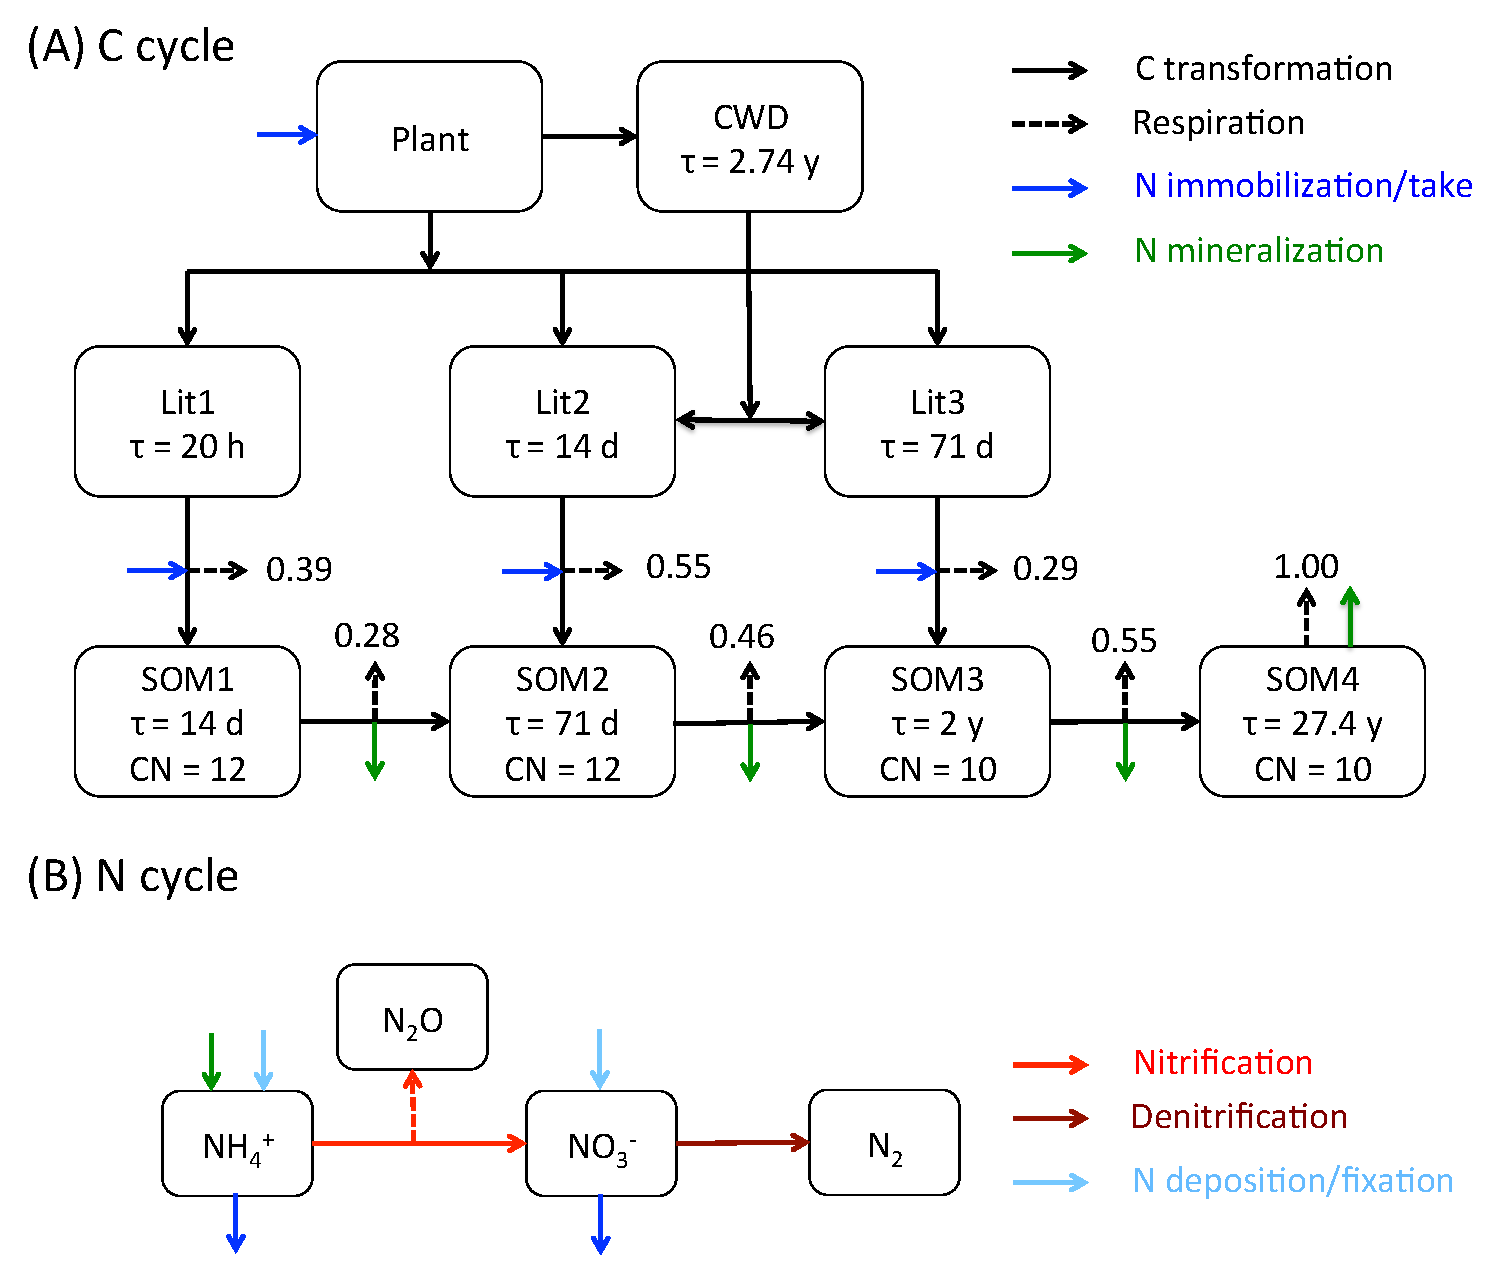
\includegraphics[width=15cm]{../figs/fig01/fig01conceptualmodel.pdf}
\caption{The reaction network for the carbon (A) and nitrogen (B) cycles
implemented in this work. The carbon cycle is modified from
\citet{Thornton2005} and \citet{Bonan2012}. $\tau$ is the turnover time, and CN
is the CN ratio in gC over gN.}
\label{fig:conceptualmodel}
\end{figure}

\begin{figure}[t]
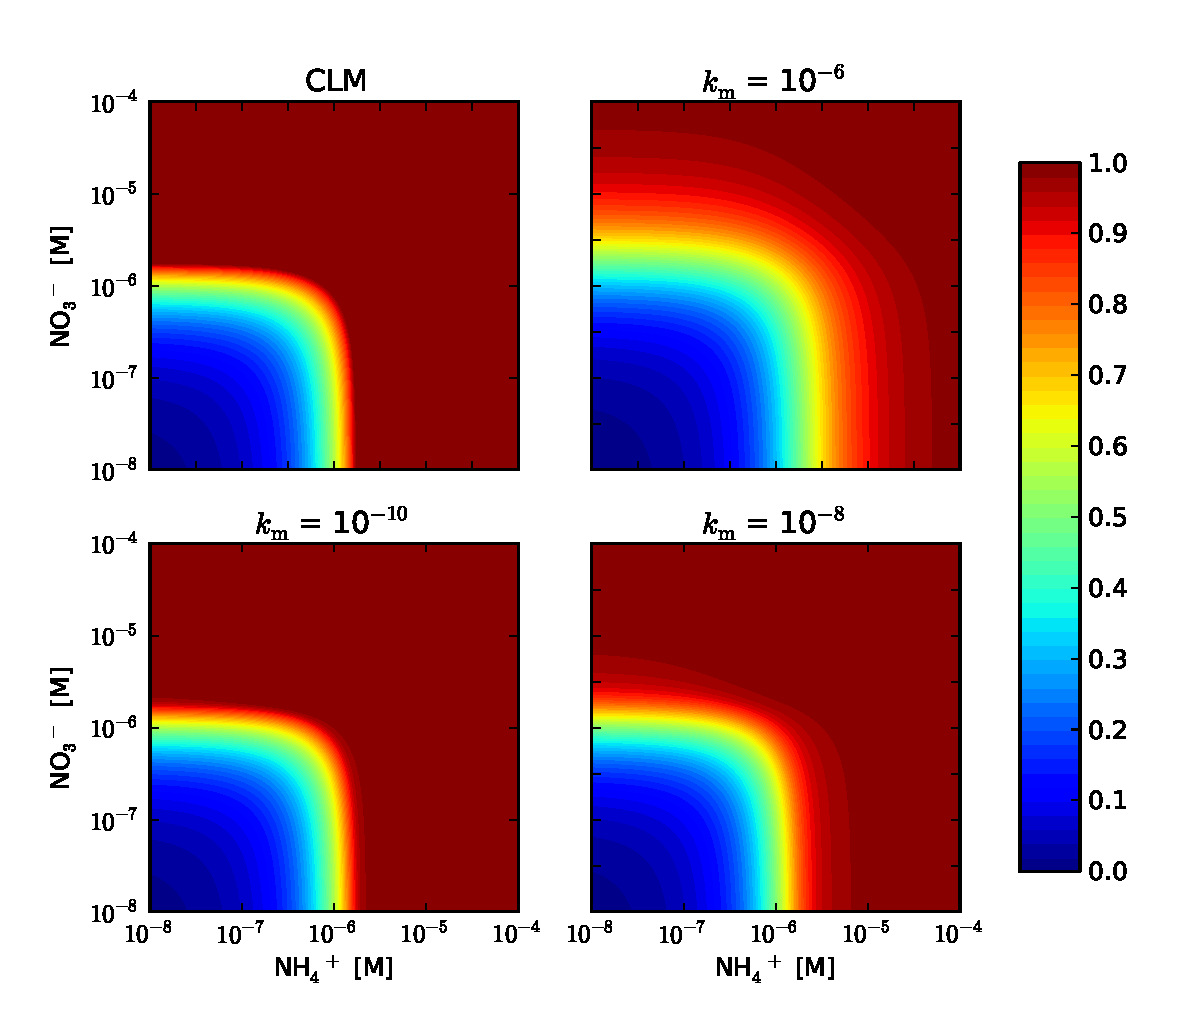
\includegraphics[width=12cm]{../figs/fig05/uptakef.pdf}
\caption{
$f_{pi}=\frac{\chem{N}_\text{take}}{\chem{N}_\text{demand}}=\max\left(1,\frac{[\chem{NH_4^+}]+[\chem{NO_3^-}]}{\chem{N}_\text{demand}}\right)$
(a) vs.
$=\frac{[\chem{NH_4^+}]}{k_\text{m}+[\chem{NH_4^+}]}+\left(1-\frac{[\chem{NH_4^+}]}{k_\text{m}+[\chem{NH_4^+}]}\right)\frac{[\chem{NO_3^-}]}{k_\text{m}+[\chem{NO_3^-}]}$
(b, c, d) in a 0.5 h time step with an uptake rate of 10$^{-9}$
\unit{M\,s^{-1}}. $f_{pi}$ for the latter representation
is less than or equal to that for the first one. The difference decreases with decreasing
half saturation $k_\text{m}$.}
\label{fig:demanddistribution}
\end{figure}

\begin{figure}[t]
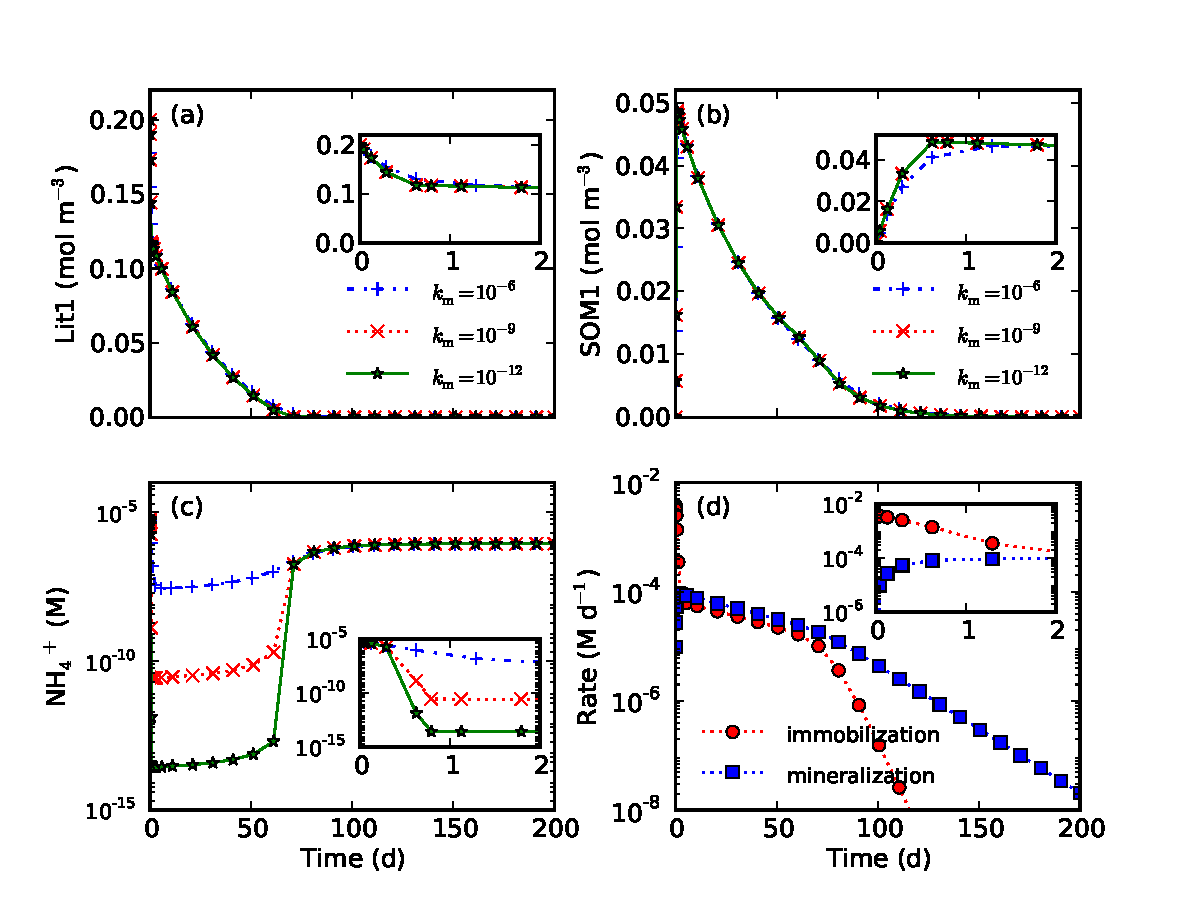
\includegraphics[width=15cm]{../figs/fig09/figdecomp.pdf}
\caption{Influence of half saturation $k_\text{m}$ on decomposition that involves both
nitrogen immobilization and mineralization. Smaller half saturation can result
in lower nitrogen concentration (c) but does not substantially impact the
calculated concentrations other than ammonium (a,b).}
\label{fig:decomp}
\end{figure}

\begin{figure}[t]
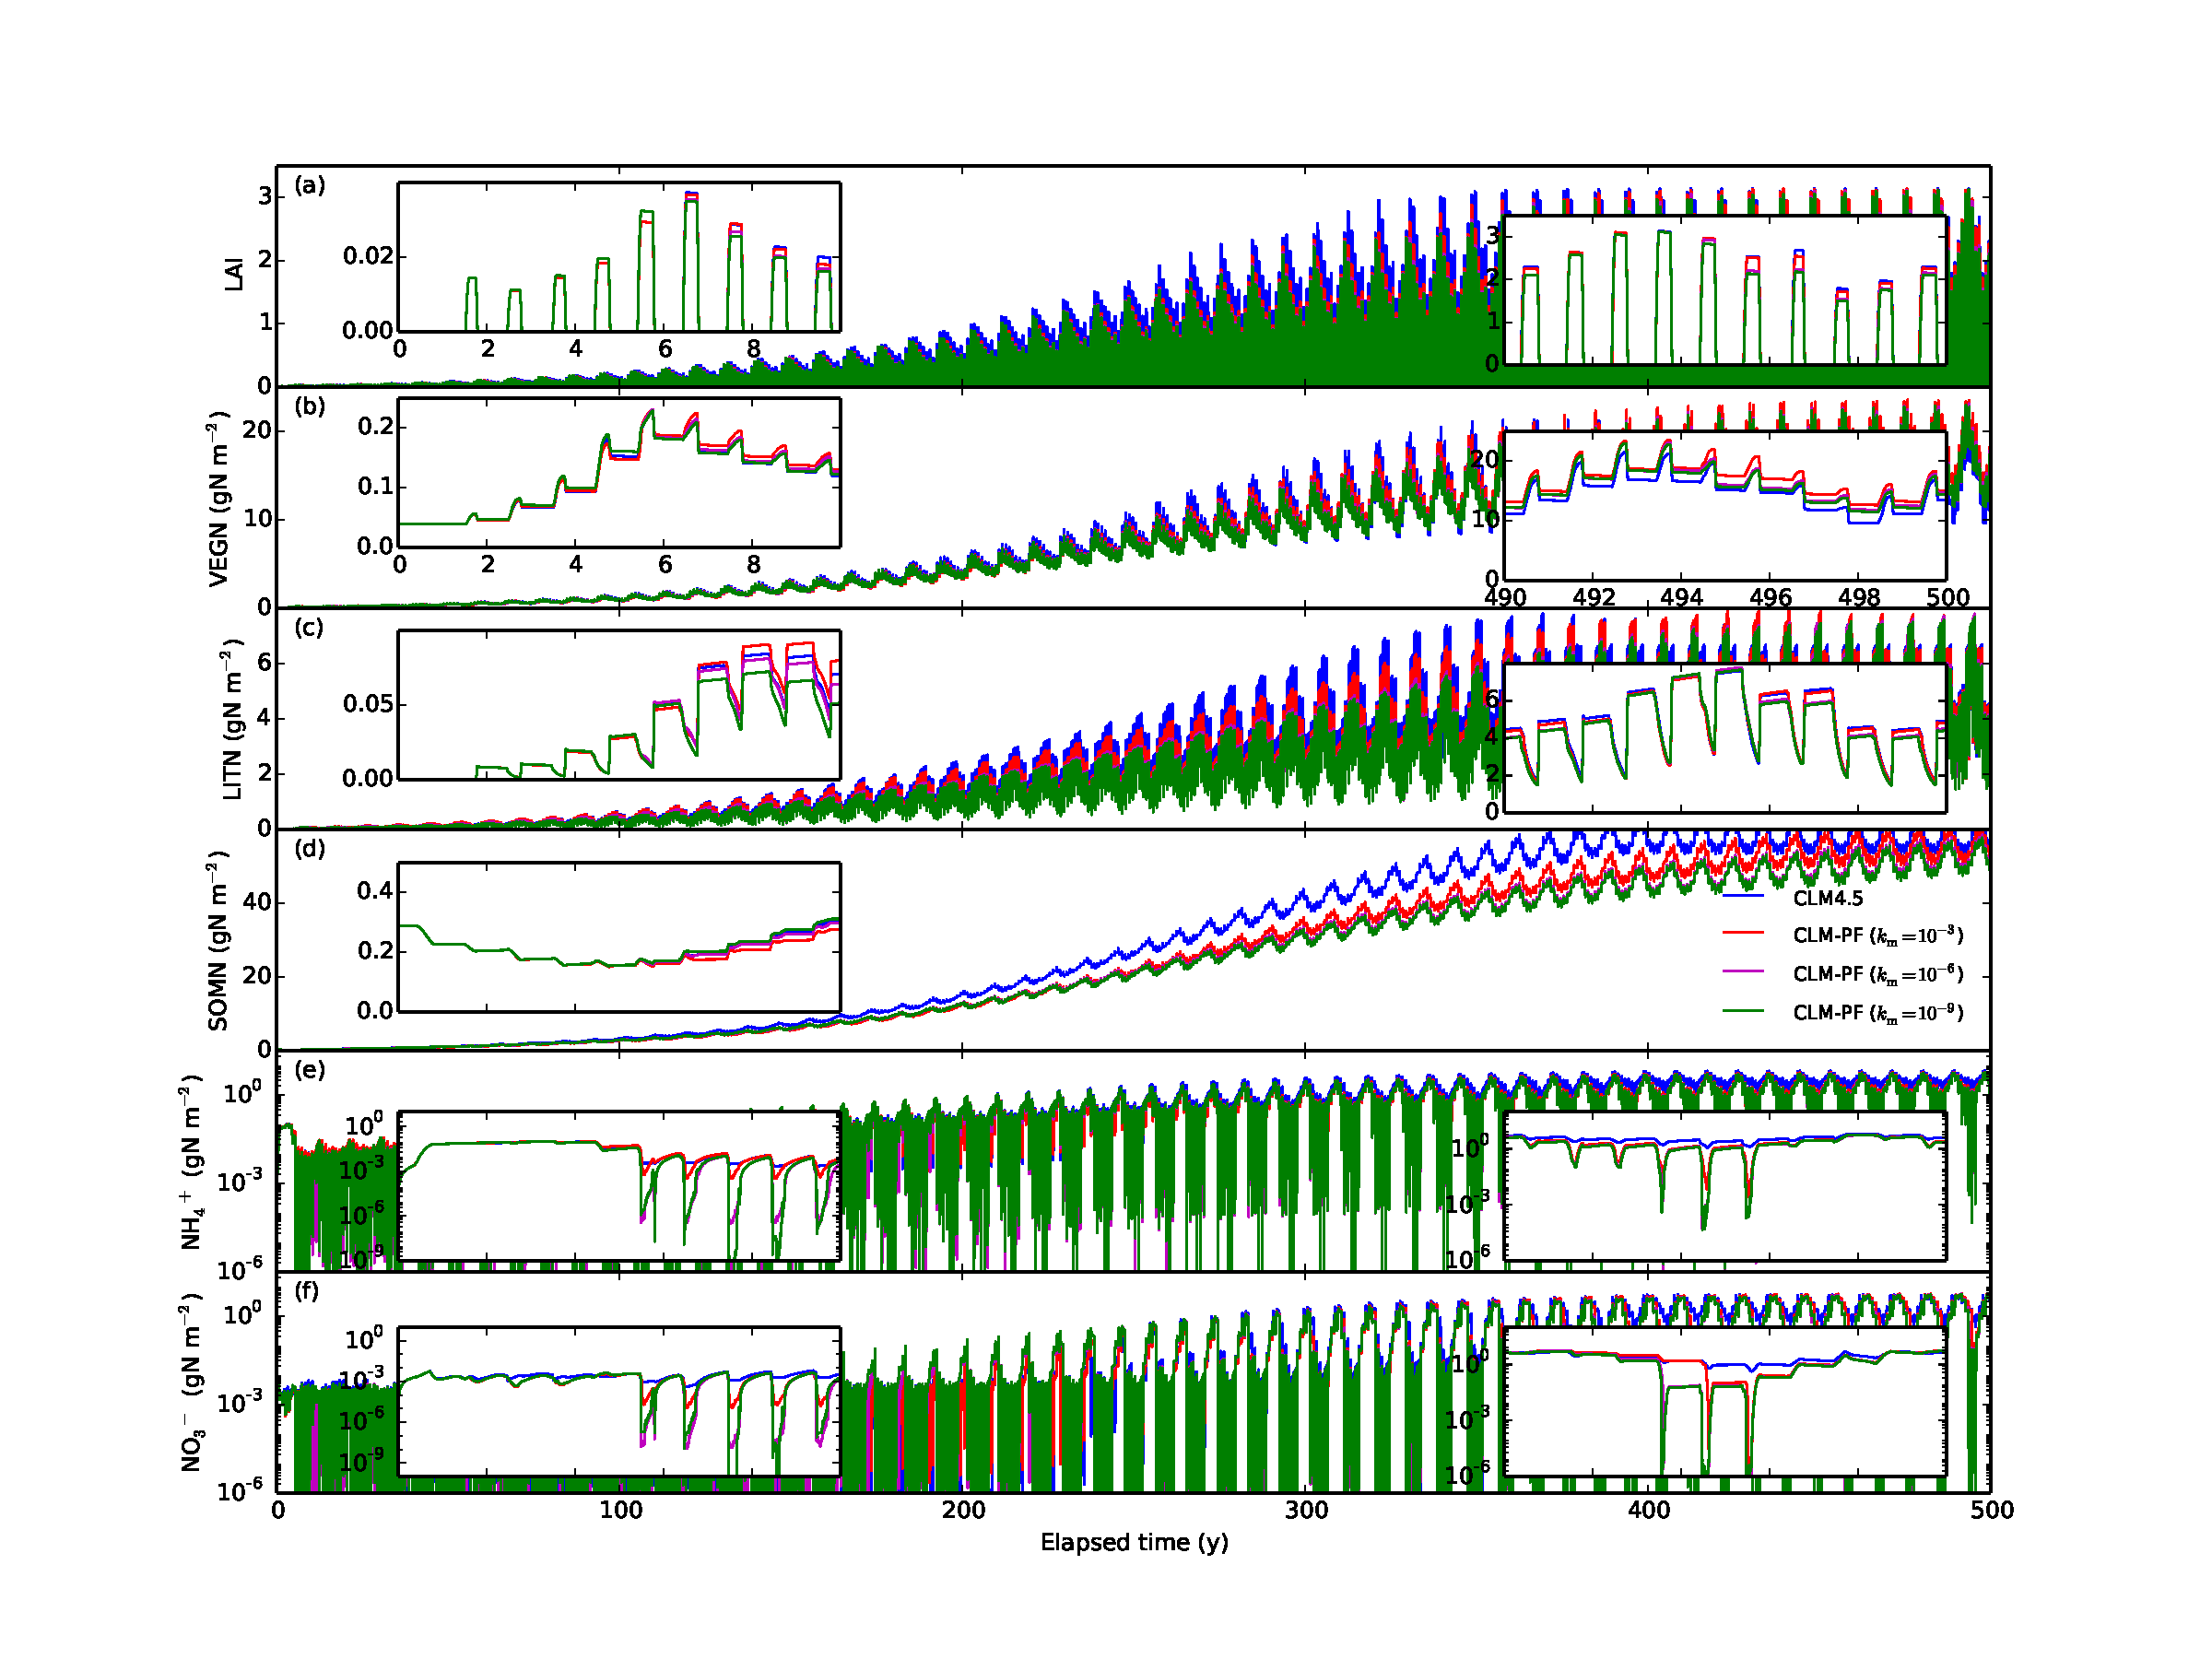
\includegraphics[width=18cm]{../figs/fig10/brw500yl.pdf}
\caption{Calculated LAI and nitrogen distribution among vegetation, litter,
SOM, \chem{NH_4^+}, and \chem{NO_3^-} pools in spin-up simulations for the US-Brw
site.}
\label{fig:brw500yl}
\end{figure}

\begin{figure}[t]
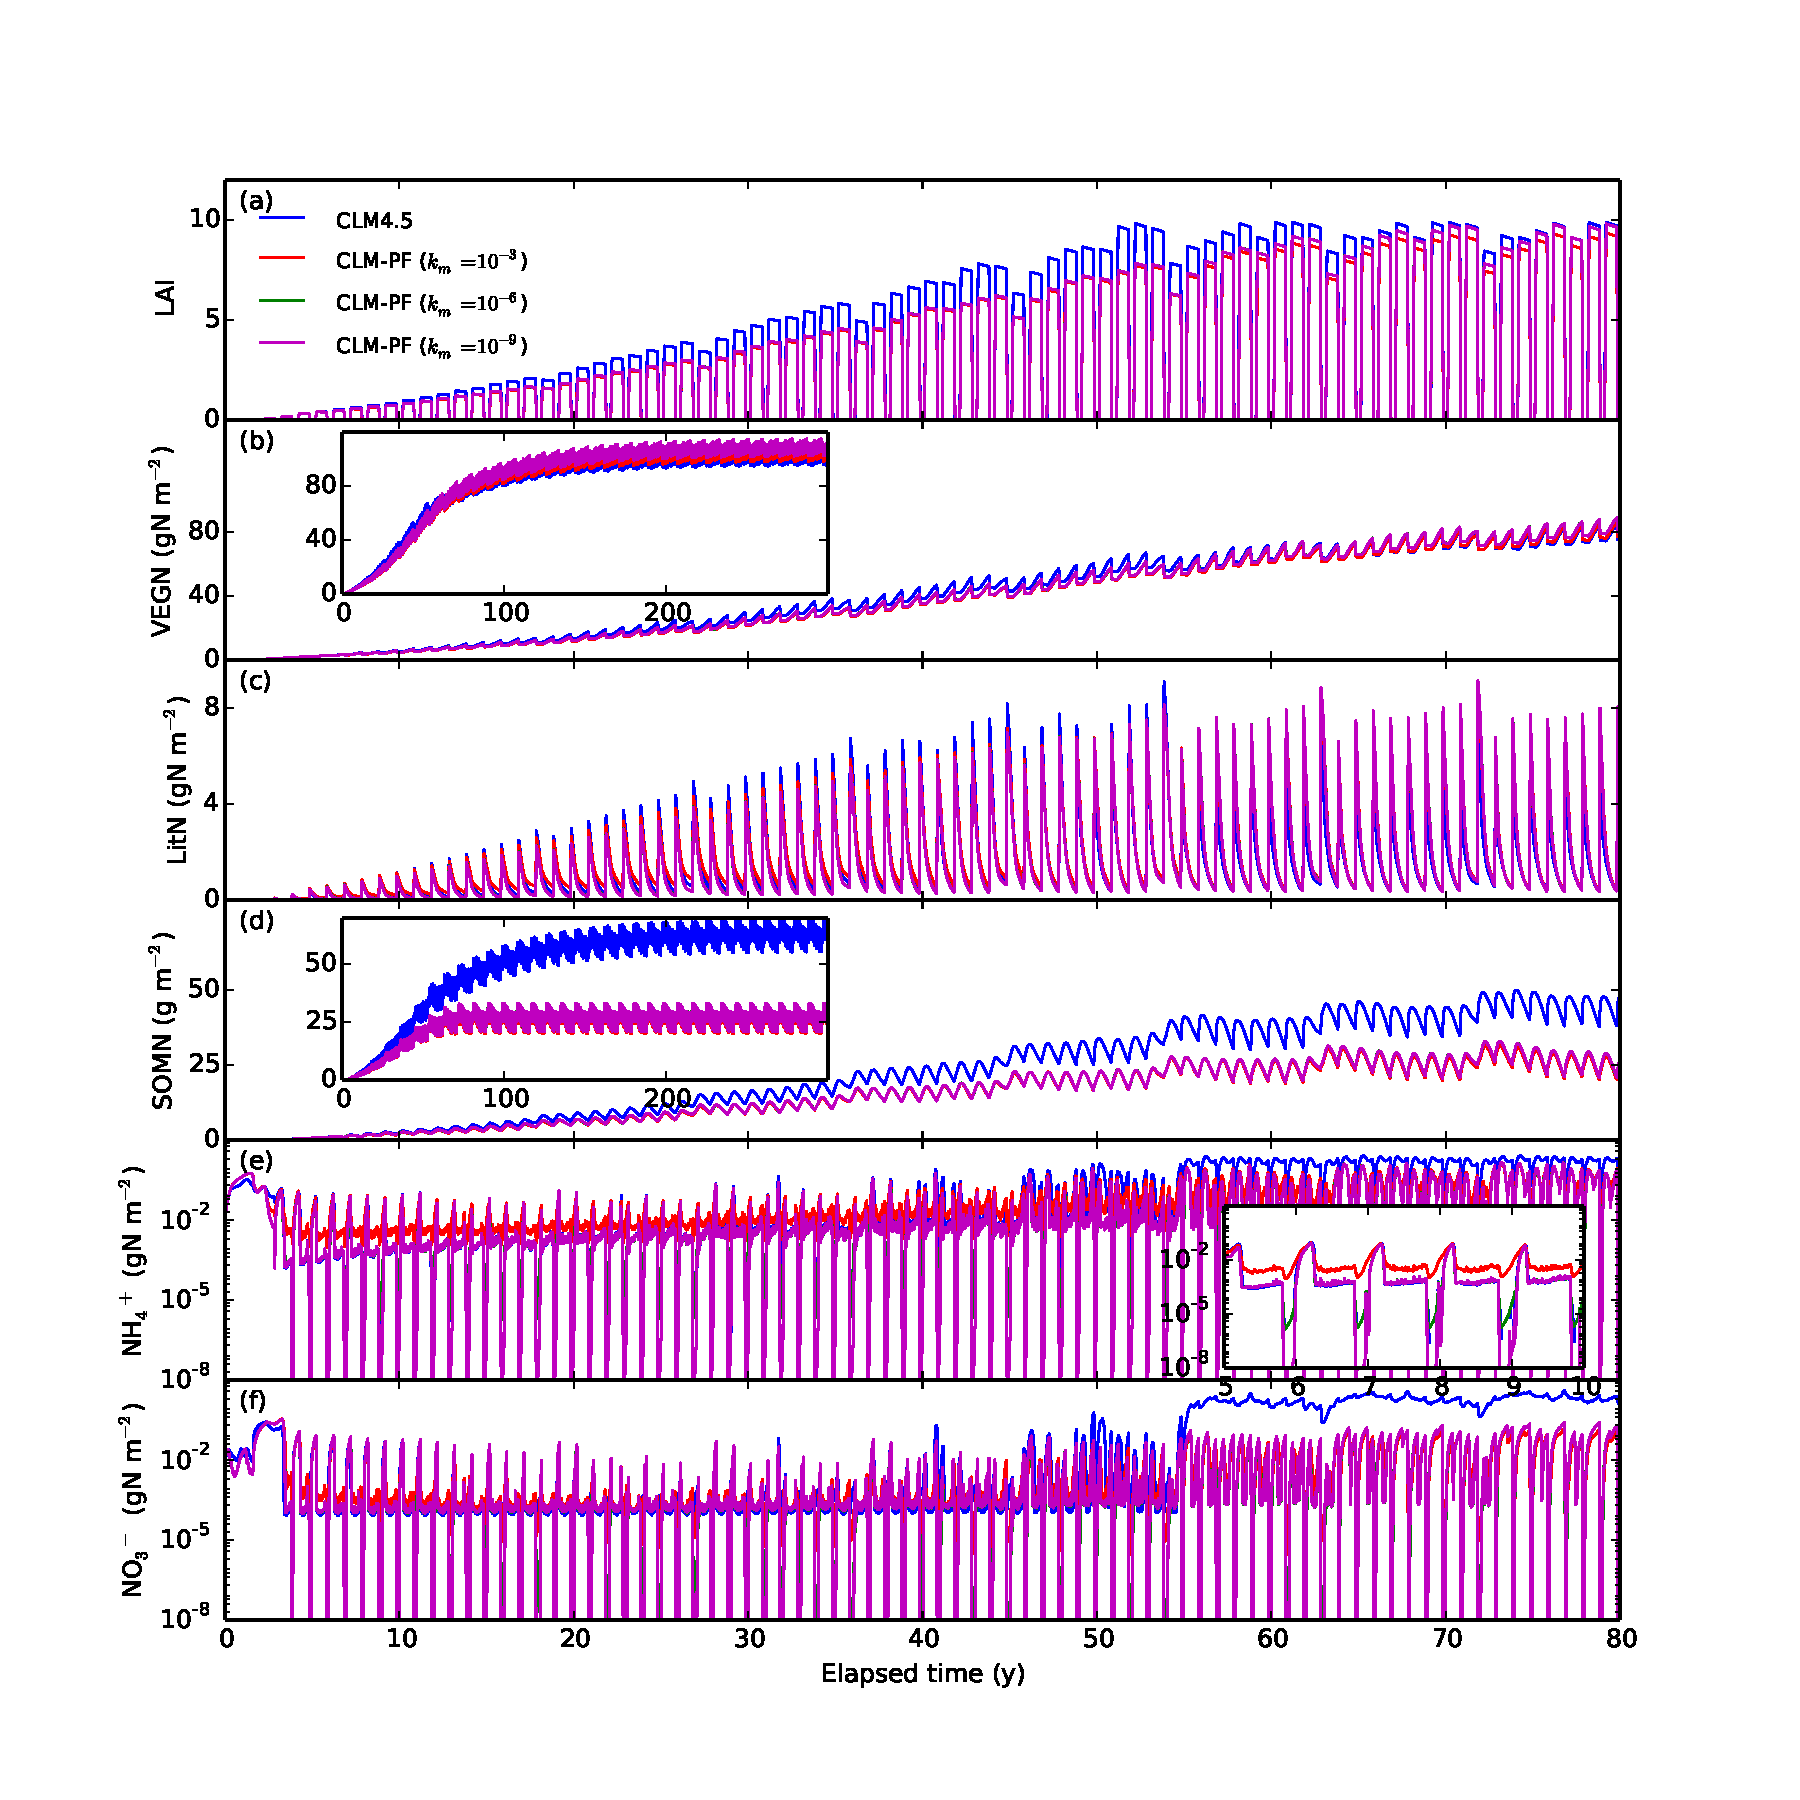
\includegraphics[width=18cm]{../figs/fig11/pit300yl.pdf}
\caption{Calculated LAI and nitrogen distribution among vegetation, litter,
SOM, \chem{NH_4^+}, and \chem{NO_3^-} pools in spin-up simulations for US-WBW
site.}
\label{fig:pit300yl}
\end{figure}

\begin{figure}[t]
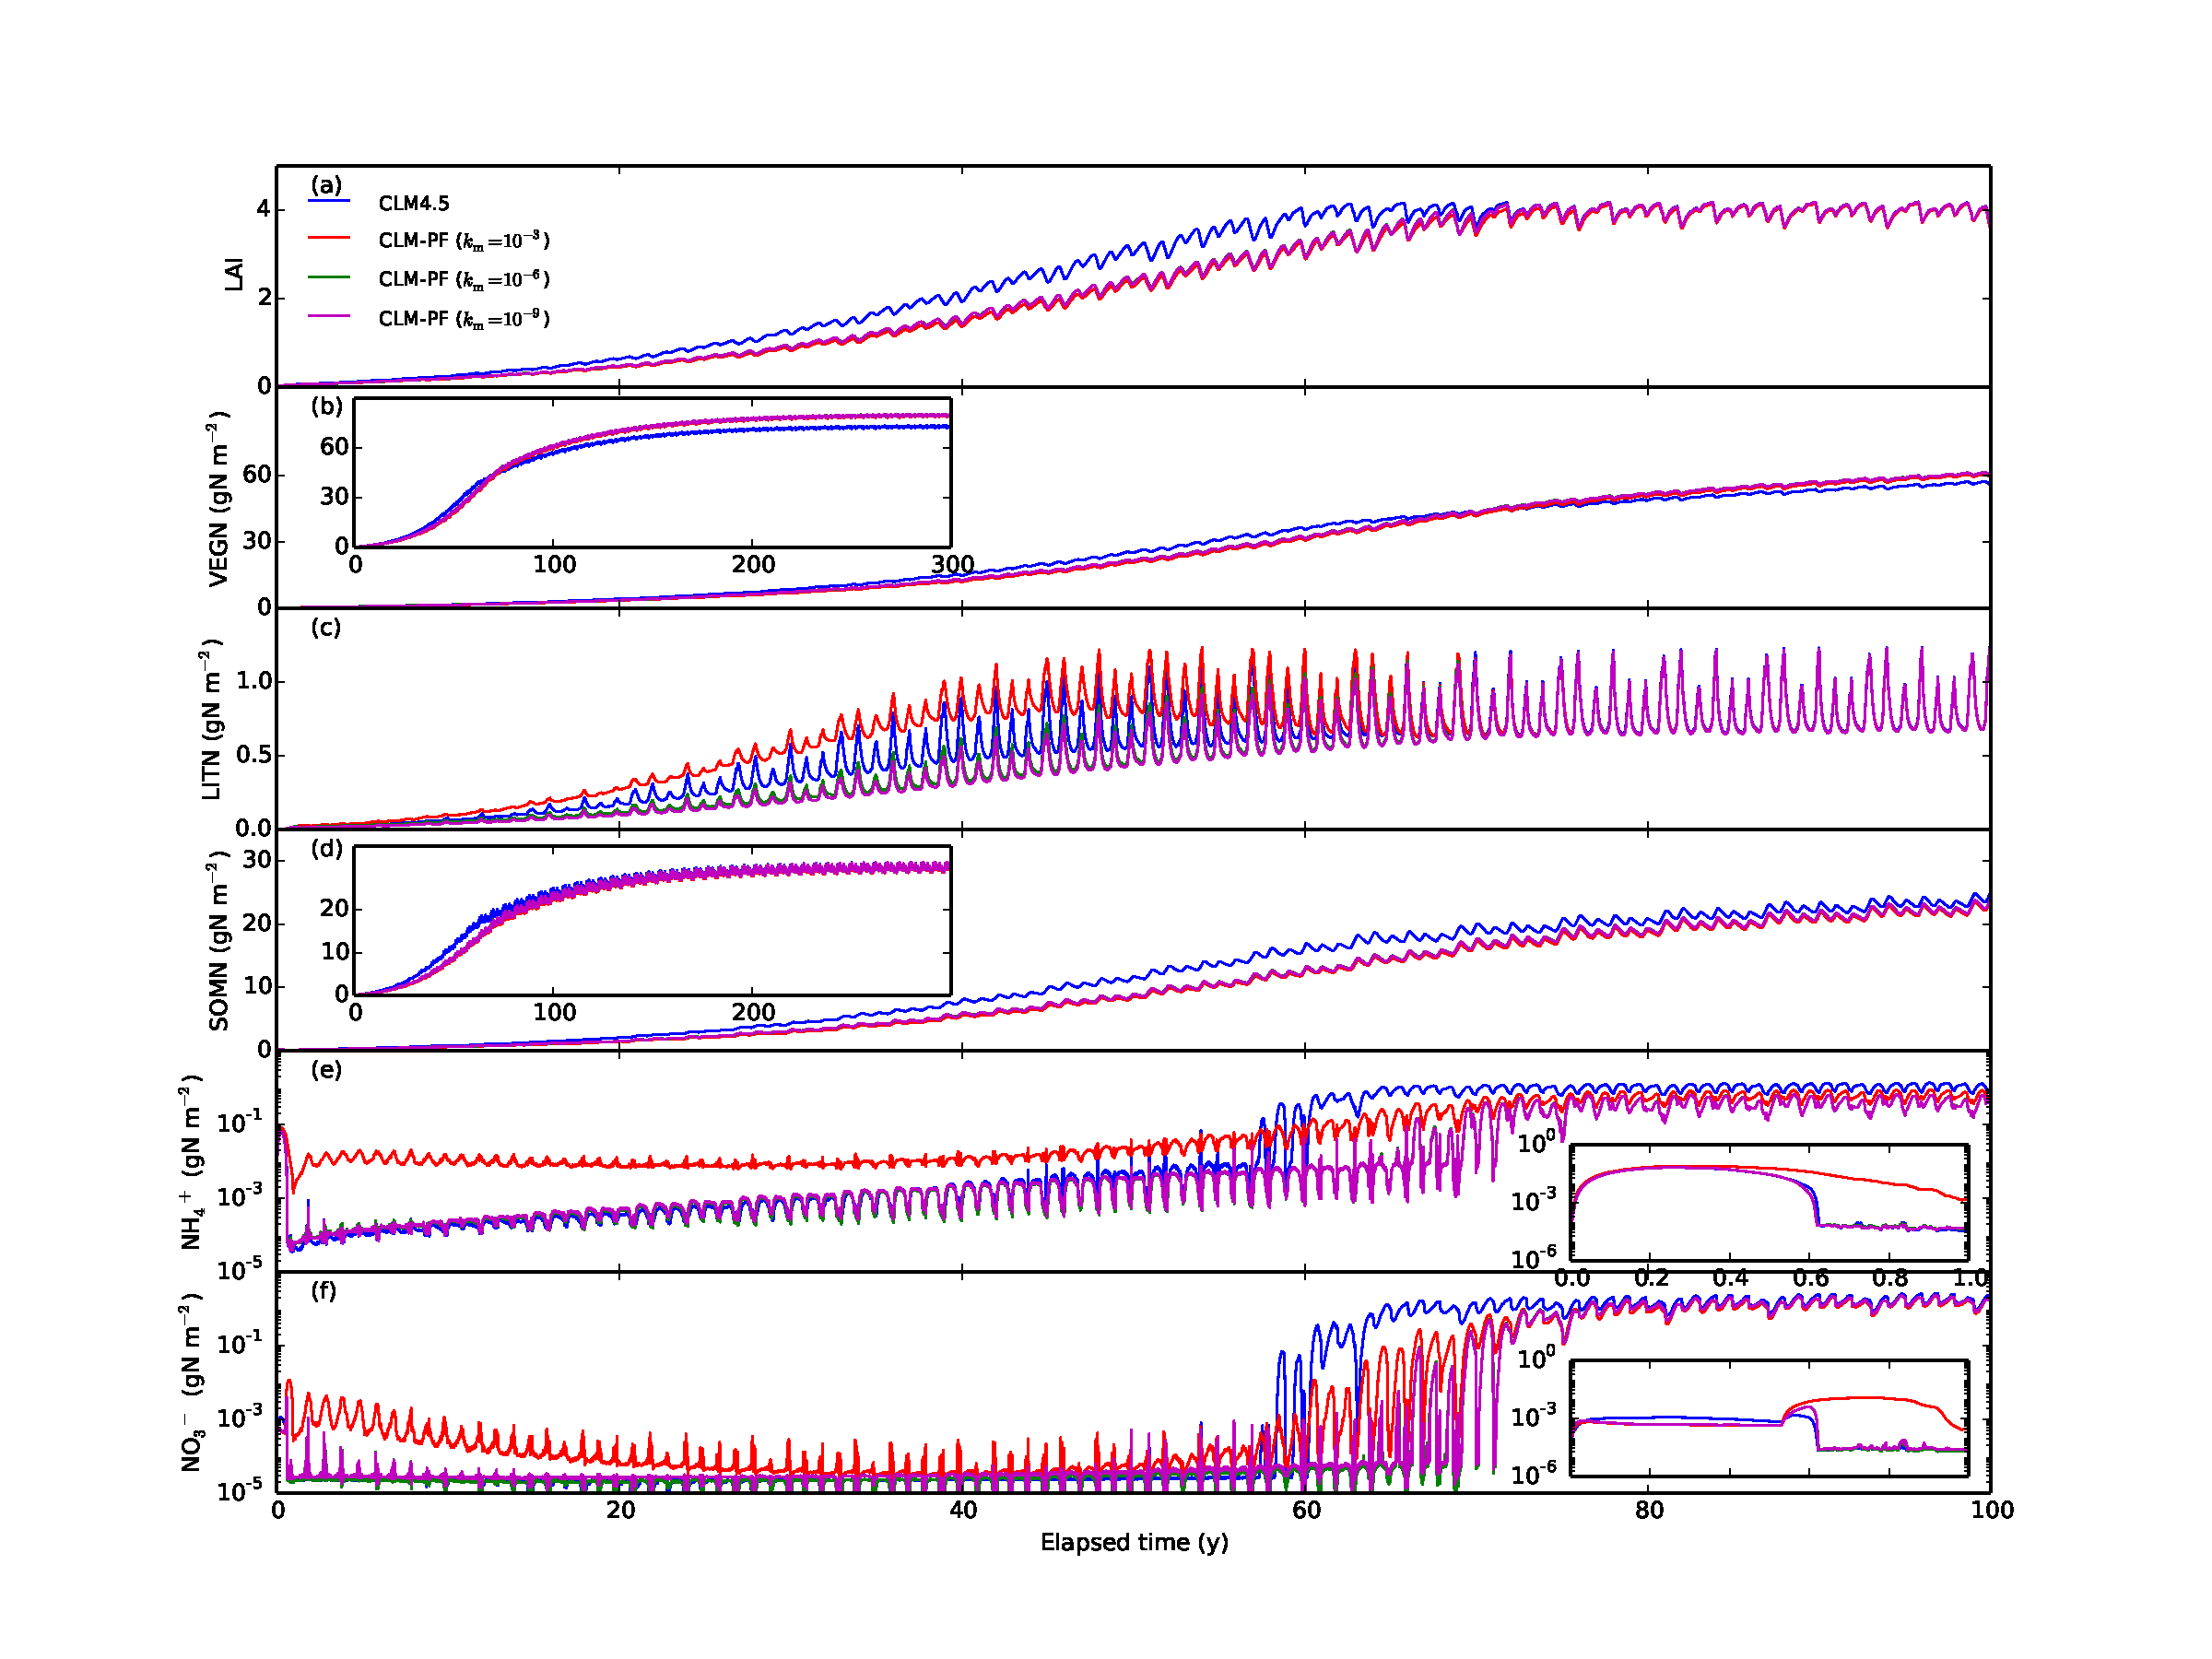
\includegraphics[width=18cm]{../figs/fig12/cax300yl.pdf}
\caption{Calculated LAI and nitrogen distribution among vegetation, litter,
SOM, \chem{NH_4^+}, and \chem{NO_3^-} pools in spin-up simulations for BR-Cax
site. }
\label{fig:cax300yl}
\end{figure}


\begin{figure}[t]
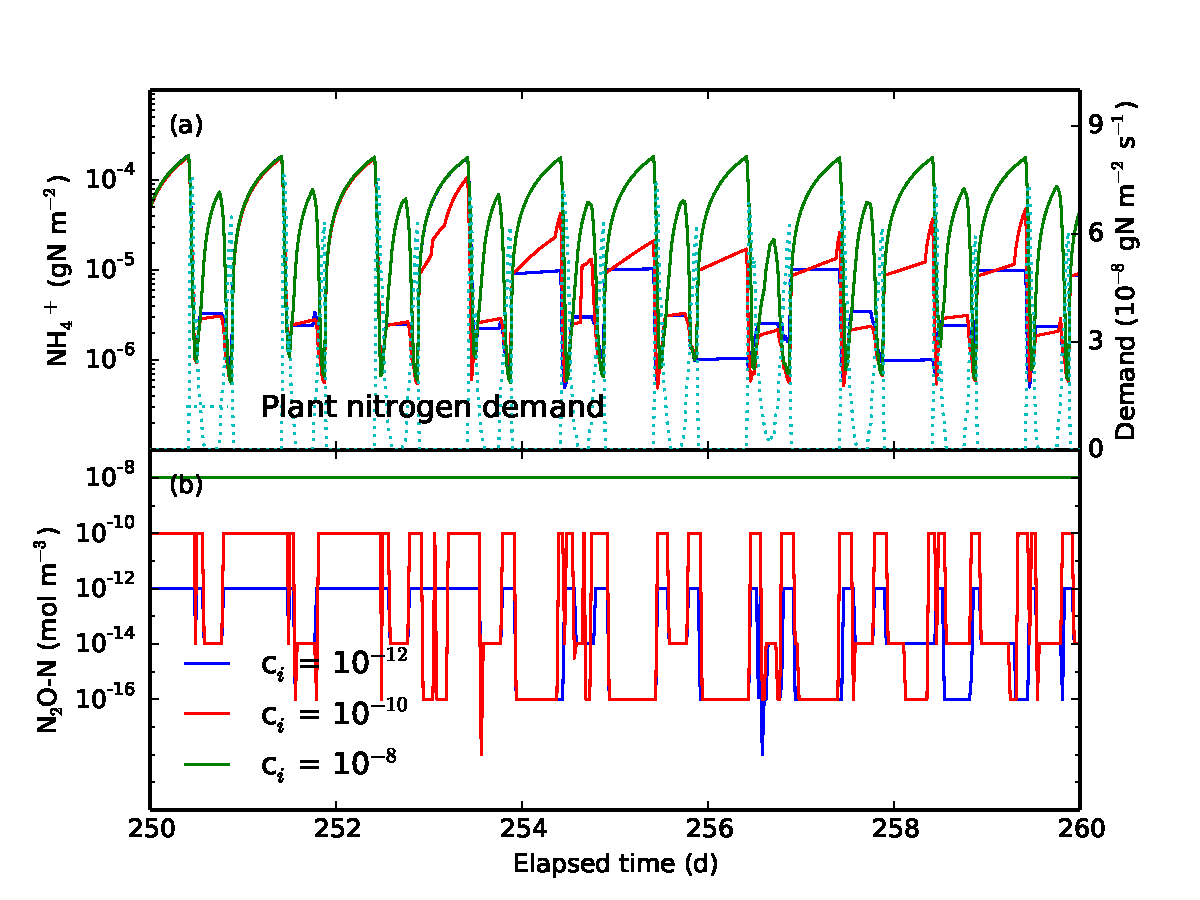
\includegraphics[width=0.8\textwidth]{../figs/fig18/cax1yn2o.pdf}
\caption{Resetting nitrous oxide concentration to $10^{-8}$, $10^{-10}$, and
$12^{-10}$ \unit{mol\,m^{-3}} in every CLM 0.5 h time step results in no
inhibition to increasing inhibition of reactions when the scaling method is
used with STOL = $10^{-8}$. \chem{N_2O-N} concentration in y-axis in (b) is the
minimum of the 10 soil layers. Numerical experiments are conducted for the
tropical site for the first year with $k_\text{m}=10^{-6}$ \unit{mol\,m^{-3}}.
See inset in Fig. (\ref{fig:cax300yl}e) for ammonium concentration in the first
year with daily data points.}
\label{fig:cax1yn2o}
\end{figure}

\begin{figure}[t]
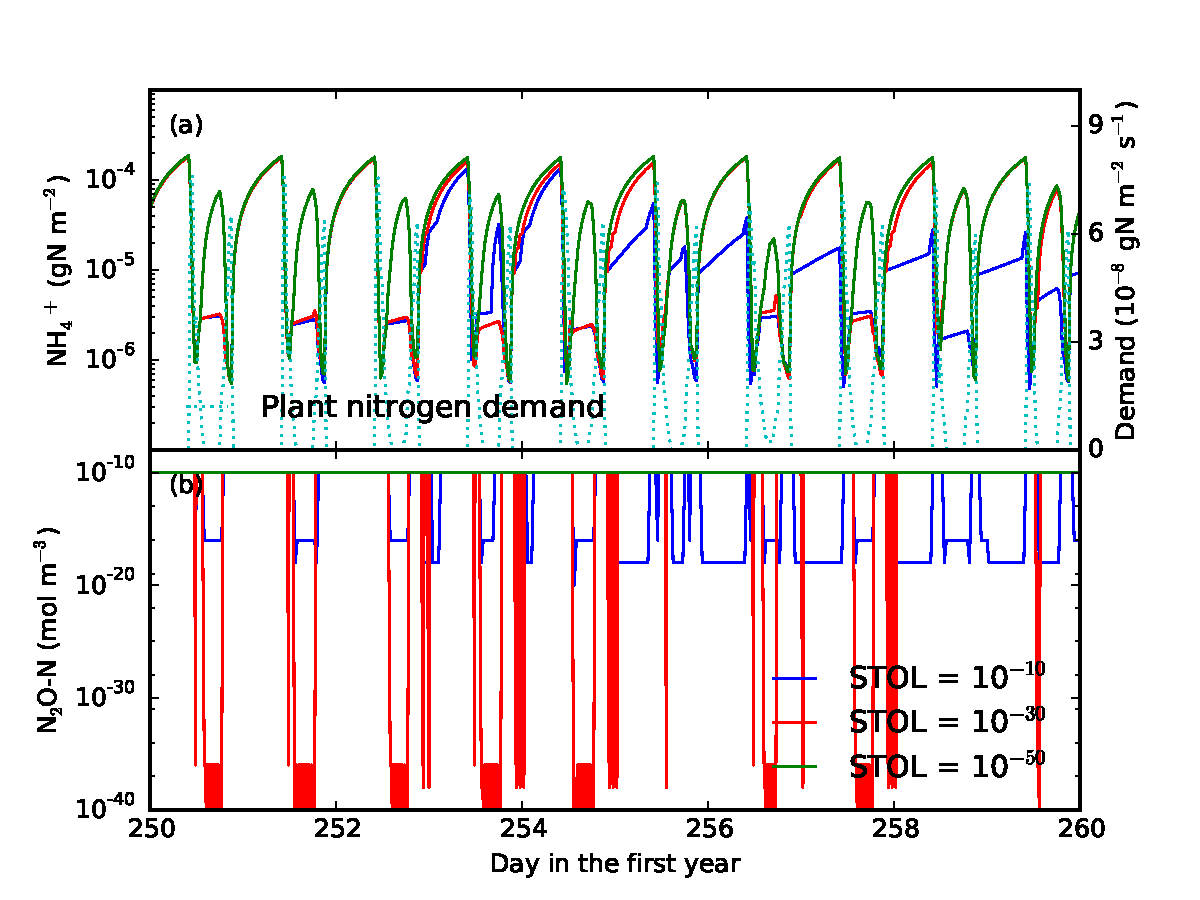
\includegraphics[width=0.8\textwidth]{../figs/fig19/cax1yn2ostol0.pdf}
\caption{Decreasing STOL can decrease and eliminate the numerical inhibition in
the case of $c_i = 10^{-10}$  \unit{mol\,m^{-3}}  in Fig. (\ref{fig:cax1yn2o}).
\chem{N_2O-N} concentration in y-axis in (b) is the minimum of the 10 soil
layers.}
\label{fig:cax1yn2osto0}
\end{figure}

\clearpage

\begin{table}[t]
\caption{Wall time for CLM-PFLOTRAN relative to CLM for spinup simulation on OIC (ORNL Institutional Cluster Phase5)}
\label{tab:computingtime}
\begin{tabular}{lrrrrrrrrr}
\tophline
Site & \multicolumn{3}{c}{Clipping}  & \multicolumn{3}{c}{Scaling} & \multicolumn{3}{c}{Log transformation} \\
\middlehline
$k_\text{m}$ & $10^{-3}$ & $10^{-6}$ & $10^{-9}$ &  $10^{-3}$ & $10^{-6}$ & $10^{-9}$ & $10^{-3}$ & $10^{-6}$ & $10^{-9}$\\
\middlehline
US-Brw & 1.28	& 1.30 &	1.30	& 1.29	& 1.29	& 1.32	& 1.45	& 1.49	& 1.72 \\
US-Pit   & 1.45	& 1.47 &	1.47	& 1.45	& 1.45	& 1.47	& 1.64	& 1.68	& 1.89 \\
BR-Cax & 1.43	& 1.49 &	1.55	& 1.44	& 1.48	& 1.52	& 1.62	& 1.66	& 1.99 \\
\bottomhline
\end{tabular}
\belowtable{CLM wall time is 29.3, 17.7, and 17.1 hour for the Arctic,
temperate, and tropical sites for a simulation duration of 1000, 600, and 600
year.}
% Table Footnotes
\end{table}


\clearpage

%% Since the Copernicus LaTeX package includes the BibTeX style file copernicus.bst,
%% authors experienced with BibTeX only have to include the following two lines:
%%
%% \bibliographystyle{copernicus}
%% \bibliography{example.bib}
%%
%% URLs and DOIs can be entered in your BibTeX file as:
%%
%% URL = {http://www.xyz.org/~jones/idx_g.htm}
%% DOI = {10.5194/xyz}


%% LITERATURE CITATIONS
%%
%% command                        & example result
%% \citet{jones90}|               & Jones et al. (1990)
%% \citep{jones90}|               & (Jones et al., 1990)
%% \citep{jones90,jones93}|       & (Jones et al., 1990, 1993)
%% \citep[p.~32]{jones90}|        & (Jones et al., 1990, p.~32)
%% \citep[e.g.,][]{jones90}|      & (e.g., Jones et al., 1990)
%% \citep[e.g.,][p.~32]{jones90}| & (e.g., Jones et al., 1990, p.~32)
%% \citeauthor{jones90}|          & Jones et al.
%% \citeyear{jones90}|            & 1990



%% FIGURES

%% ONE-COLUMN FIGURES

%%f
%\begin{figure}[t]
%\includegraphics[width=8.3cm]{FILE NAME}
%\caption{TEXT}
%\end{figure}
%
%%% TWO-COLUMN FIGURES
%
%%f
%\begin{figure*}[t]
%\includegraphics[width=12cm]{FILE NAME}
%\caption{TEXT}
%\end{figure*}
%
%
%%% TABLES
%%%
%%% The different columns must be seperated with a & command and should
%%% end with \\ to identify the column brake.
%
%%% ONE-COLUMN TABLE
%
%%t
%\begin{table}[t]
%\caption{TEXT}
%\begin{tabular}{column = lcr}
%\tophline
%
%\middlehline
%
%\bottomhline
%\end{tabular}
%\belowtable{} % Table Footnotes
%\end{table}
%
%%% TWO-COLUMN TABLE
%
%%t
%\begin{table*}[t]
%\caption{TEXT}
%\begin{tabular}{column = lcr}
%\tophline
%
%\middlehline
%
%\bottomhline
%\end{tabular}
%\belowtable{} % Table Footnotes
%\end{table*}
%
%
%%% NUMBERING OF FIGURES AND TABLES
%%%
%%% If figures and tables must be numbered 1a, 1b, etc. the following command
%%% should be inserted before the begin{} command.
%
%\addtocounter{figure}{-1}\renewcommand{\thefigure}{\arabic{figure}a}
%
%
%%% MATHEMATICAL EXPRESSIONS
%
%%% All papers typeset by Copernicus Publications follow the math typesetting regulations
%%% given by the IUPAC Green Book (IUPAC: Quantities, Units and Symbols in Physical Chemistry,
%%% 2nd Edn., Blackwell Science, available at: http://old.iupac.org/publications/books/gbook/green_book_2ed.pdf, 1993).
%%%
%%% Physical quantities/variables are typeset in italic font (t for time, T for Temperature)
%%% Indices which are not defined are typeset in italic font (x, y, z, a, b, c)
%%% Items/objects which are defined are typeset in roman font (Car A, Car B)
%%% Descriptions/specifications which are defined by itself are typeset in roman font (abs, rel, ref, tot, net, ice)
%%% Abbreviations from 2 letters are typeset in roman font (RH, LAI)
%%% Vectors are identified in bold italic font using \vec{x}
%%% Matrices are identified in bold roman font
%%% Multiplication signs are typeset using the LaTeX commands \times (for vector products, grids, and exponential notations) or \cdot
%%% The character * should not be applied as mutliplication sign
%
%
%%% EQUATIONS
%
%%% Single-row equation
%
%\begin{equation}
%
%\end{equation}
%
%%% Multiline equation
%
%\begin{align}
%& 3 + 5 = 8\\
%& 3 + 5 = 8\\
%& 3 + 5 = 8
%\end{align}
%
%
%%% MATRICES
%
%\begin{matrix}
%x & y & z\\
%x & y & z\\
%x & y & z\\
%\end{matrix}
%
%
%%% ALGORITHM
%
%\begin{algorithm}
%\caption{}
%\label{a1}
%\begin{algorithmic}
%
%\end{algorithmic}
%\end{algorithm}
%
%
%%% CHEMICAL FORMULAS AND REACTIONS
%
%%% For formulas embedded in the text, please use \chem{}
%
%%% The reaction environment creates labels including the letter R, i.e. (R1), (R2), etc.
%
%\begin{reaction}
%%% \rightarrow should be used for normal (one-way) chemical reactions
%%% \rightleftharpoons should be used for equilibria
%%% \leftrightarrow should be used for resonance structures
%\end{reaction}
%
%
%%% PHYSICAL UNITS
%%%
%%% Please use \unit{} and apply the exponential notation

%\input{appendix}

\appendix

\section{CLM biogeochemical reactions and rates}
\label{sec:clmbgc}
\subsection{CLM-CN decomposition}
\label{section:bgc}

The CLM-CN decomposition cascade consists of three litter pools with variable
CN ratios, four soil organic matter (SOM) pools with constant CN ratios, and
seven reactions \citep{Bonan2012,Oleson2013,Thornton2005}. The reaction can be
described by
\begin{reaction}
\chem{CN_u} \rightarrow (1 - f) \chem{CN_d} + f \chem{CO_2} + n \chem{N},
\label{rxn:decomp}
\end{reaction}
with \chem{CN_u} and \chem{CN_d} as the upstream and downstream pool (molecular
formula, for 1 mol upstream and downstream pool, there is u and d mol N),
\chem{N} as either \chem{NH_4^+} or \chem{NO_3^-}, \textit{f} as the
respiration fraction, and \textit{n} = u $-$ (1 $-$ \textit{f})d. The rate is
\begin{equation}
\frac{d [\chem{CN_u}]}{d t} = - k_\text{d} f_\text{T} f_\text{w} [\chem{CN_u}],
\label{eq:decomprate}
\end{equation}
with $\textit{k}_\text{d}$ as the rate coefficient and $\textit{f}_\text{T}$
and $\textit{f}_\text{w}$ as the temperature and moisture response functions.
%\begin{equation}
%f_T = Q_{10}^{(T - 25)/10}, 
%\end{equation}
%and
%\begin{equation}
%f_w = \ln(\psi)Q_{10}^{(T - 25)/10}, 
%\end{equation}
With a constant CN ratio, the decomposition reactions for the four SOM pools are 
\begin{reaction}
\chem{SOM1} \rightarrow 0.72 \chem{SOM2} + 0.28 \chem{CO_2} + 0.02 \chem{N},
\label{rxn:som1}
\end{reaction}
\begin{reaction}
\chem{SOM2} \rightarrow 0.54 \chem{SOM3} + 0.46 \chem{CO_2} + 0.025143 \chem{N},
\label{rxn:som2}
\end{reaction}
\begin{reaction}
\chem{SOM3} \rightarrow 0.45 \chem{SOM4} + 0.55 \chem{CO_2} + 0.047143 \chem{N},
\label{rxn:som3}
\end{reaction}
and
\begin{reaction}
\chem{SOM4} \rightarrow \chem{CO_2} + 0.085714 \chem{N}.
\label{rxn:som4}
\end{reaction}
The exact stoichiometric coefficients are calculated in the code using values
for respiration factor, CN ratio, and molecular weight specified in the input
file.

CLM4.5 has an option to separate \chem{N} into \chem{NH_4^+} and \chem{NO_3^-}.
The \chem{N} mineralization product is \chem{NH_4^+}.
% see CNNStateUpdate1Mod.F90 line 359-391. 

As the CN ratio is variable for the three litter pools, litter N pools need to
be tracked such that reaction (\ref{rxn:decomp}) becomes
\begin{reaction}
\chem{LitC} + u \chem{LitN} \rightarrow (1 - f) \chem{CN_d} + f \chem{CO_2} + n \chem{N}, 
\label{rxn:lit}
\end{reaction}
with $\textit{u}$ = [LitN]/[LitC]. The three litter decomposition reactions are
\begin{reaction}
\chem{Lit1C} + u_1 \chem{Lit1N} \rightarrow 0.41 \chem{SOM1} + 0.39 \chem{CO_2} + (u_1 - 0.029286) \chem{N},
\label{rxn:lit1}
\end{reaction}
\begin{reaction}
\chem{Lit2C} + u_2 \chem{Lit2N} \rightarrow 0.45 \chem{SOM2} + 0.55 \chem{CO_2} + (u_2 - 0.032143) \chem{N},
\label{rxn:lit2}
\end{reaction}
and
\begin{reaction}
\chem{Lit3C} + u_3 \chem{Lit3N} \rightarrow 0.71 \chem{SOM3} + 0.29 \chem{CO_2} + (u_3 - 0.060857) \chem{N}.
\label{rxn:lit3}
\end{reaction}
As the CN ratio of the litter pools is generally  high, $u_1$, $u_2$, and $u_3$
are usually small, and $n$ in these reactions (e.g., $n_1 = u_1 - 0.029286$ for
\chem{Lit1}) is normally negative. Namely, these reactions consume (immobilize)
\chem{N}, which can be \chem{NH_4^+}, \chem{NO_3^-}, or both. 

\subsection{Nitrification}
The nitrification reaction to produce \chem{NO_3^-} is 
\begin{reaction}
\chem{NH_4^+} + \cdots \rightarrow \chem{NO_3^-} + \cdots
\label{rxn:nitr2no3}
\end{reaction}
with $\cdots$ for additional reactants and products to balance the reaction. The
rate is (Dickinson et al., 2002) 
\begin{equation}
\frac{d [\chem{NH_4^+}]}{d t} = -\frac{d
[\chem{NO_3^-]}}{d t} = -k_\text{n} f_\text{T} f_\text{w}
[\chem{NH_4^+}].
\label{eq:nitr2no3}
\end{equation}
The nitrification reaction to produce $\chem{N_2O}$ is
\begin{reaction}
\chem{NH_4^+} + \cdots \rightarrow 0.5 \chem{N_2O} + \cdots,
\label{rxn:nitr2n2o}
\end{reaction}
with one component related to decomposition as %when
%$\chem{NH_4^+}$ is low ( < 3 $\mu \text{gN g}^{-1}$) as 
\begin{equation}
\frac{d [\chem{NH_4^+}]}{d t} = -2\frac{d
[\chem{N_2O}]}{d t} = -f_\text{nm} f_\text{T} f_\text{w}
f_\text{pH}\max(R_\text{nm},0)
\label{eq:nitr2n2odecomp}
\end{equation}
with $f_\text{nm}$ as a fraction \citep{Parton1996} and $R_\text{nm}$ as the
net \chem{N} mineralization rate,  
\begin{equation}
R_\text{nm}=\sum_{i} n_iR_i,
\label{eq:netnmin}
\end{equation}
where $R_i$ denotes the rate of reaction (\ref{rxn:som1}, \ref{rxn:som2},
\ref{rxn:som3}, \ref{rxn:som4}, \ref{rxn:lit1}, \ref{rxn:lit2},
\ref{rxn:lit3}).
The second component is \citep{Parton1996} %relates to excessive \chem{NH_4^+}
%(> 3 $\mu$gN g$^{-1}$) 
\begin{equation} 
\frac{d [\chem{NH_4^+}]}{d t} = -2\frac{d
[\chem{N_2O}]}{d t} = -k_\text{n2o} f_\text{T} f_\text{w}
f_\text{pH}(1-e^{-0.0105[\chem{NH_4^+}]}).
\label{eq:nitr2n2oexess}
\end{equation}
Ignoring the high-order terms and moving the unit conversion factor into
$k_\text{n2o}$, it can be simplified as a first-order
rate as
\begin{equation} 
\frac{d [\chem{NH_4^+}]}{d t} = -2\frac{d
[\chem{N_2O}]}{d t} = -k_\text{n2o} f_\text{T} f_\text{w}
f_\text{pH}[\chem{NH_4^+}].
\label{eq:nitr2n2oexesssimple}
\end{equation}

\subsection{Denitrification} 
The denitrification reaction is
\begin{reaction}
\chem{NO_3^-} + \cdots \rightarrow 0.5 \chem{N_2} + \cdots
\label{rxn:deni}
\end{reaction}
with rate \citep{Dickinson2002} 
\begin{equation} 
\frac{d [\chem{NO_3^-}]}{d t} = -2\frac{d
[\chem{N_2}]}{d t} = -k_\text{deni} f_\text{T} f_\text{w}
f_\text{pH}[\chem{NO_3^-}].
\label{eq:deni}
\end{equation}

\subsection{Plant nitrogen uptake}
The plant nitrogen uptake reaction can be written as
\begin{reaction}
\chem{NH_4^+} + \cdots \rightarrow \chem{PlantA} + \cdots
\label{rxn:plantatake}
\end{reaction}
and
\begin{reaction}
\chem{NO_3^-} + \cdots \rightarrow \chem{PlantN} + \cdots.
\label{rxn:plantntake}
\end{reaction}
The rate is specified by CLM (plant nitrogen demand) and assumed to be
constant in each half-hour time step. 

\subsection{Demand-based competition and demand distribution between ammonium and nitrate}
\label{sec:demandbasedcompetition}
Denote $R_{d,p}$ and $R_{d,i}$ as the potential plant,
immobilization, nitrification, and denitrification demand (rate);
$R_{a,tot}=R_{d,p}+R_{d,i}$ as the total \chem{NH_4^+} demand; and
$R_{n,tot}$ as the total \chem{NO_3^-} demand. CLM uses a demand-based
competition approach to split the available sources in proportion to the demand
rates to meet the demands \citep{Oleson2013,Thornton2005}. Specifically, for
each time step, if $R_{a,tot}\Delta t \leq [\chem{NH_4^+}]$, the uptakes are
equal to potential demands, and $R_{n,tot}$ = 0; otherwise, the uptakes for
\chem{NH_4^+} are [\chem{NH_4^+}]$R_{d,p}/R_{a,tot}\Delta t$ and
[\chem{NH_4^+}]$R_{d,i}/R_{a,tot}\Delta t$ for plants and immobilization;
$R_{n,tot}=R_{a,tot}-[\chem{NH_4^+}]/\Delta t$. If $R_{n,tot}\Delta t <
[\chem{NO_3^-}]$, all of the remaining
demand $R_{n,tot}$ is met with available \chem{NO_3^-}. Otherwise, available
\chem{NO_3^-} is split to meet the remaining plant, immobilization, and
denitrification demands in proportion to their rates. 

\section{Implicit time stepping and Newton-Raphson iteration}
\label{sec:newton}
Ignoring equilibrium reactions and transport for simplicity of discussion in
this work, PFLOTRAN solves the ordinary differential equation,
\begin{equation}
\label{eq:cde}
{d \mathbf{c}}/{d t} = \mathbf{R}(\mathbf{c}) + \mathbf{F},
\end{equation}
with $\mathbf{c}$ as the concentration vector, $\mathbf{R}$ as the kinetic reaction rate, and $\mathbf{F}$ as the fluxes (e.g., nitrogen deposition). 
Discretizing Eq. (\ref{eq:cde}) in time using the backward Euler method, 
\begin{equation}
{(\mathbf{c}^{k+1} - \mathbf{c}^k)}/{\Delta t} = \mathbf{R}(\mathbf{c}^{k+1}) + \mathbf{F}^k.
\label{eq:cdedis}
\end{equation}
Solving the equation  using the Newton-Raphson method, we denote the residual as
\begin{equation}
\mathbf{f}(\mathbf{c}^{k+1,p} )=(\mathbf{c}^{k+1,p}-\mathbf{c}^k)/\Delta t-\mathbf{R}(\mathbf{c}^{k+1,p})-\mathbf{F}^k,
\label{eq:residual}
\end{equation}
and Jacobian as
\begin{equation}
\mathbf{J} = \frac{\partial \mathbf{f}(\mathbf{c}^{k+1,p})}{\partial \mathbf{c}^{k+1,p}},
\label{eq:jacobian}
\end{equation}
with $p$ as the iteration counter, the update is
\begin{equation}
\delta \mathbf{c}^{k+1,p+1}= -\mathbf{J}^{-1} \mathbf{f} (\mathbf{c}^{k+1,p}),
\label{eq:axb}
\end{equation}
and the iteration equation is
\begin{equation}
\mathbf{c}^{k+1,p+1}=\mathbf{c}^{k+1,p}+\delta \mathbf{c}^{k+1,p+1}.
\label{eq:update}
\end{equation}
The iteration continues until either the residual
$\mathbf{f}(\mathbf{c}^{k+1,p+1} )$ or the update $\delta
\mathbf{c}^{k+1,p+1}$ is less than a specified tolerance. Specifically,
\begin{equation}
\|\mathbf{f}(\mathbf{c}^{k+1,p+1} )\|_2 < \text{ATOL},
\label{eq:atol}
\end{equation}
\begin{equation}
\frac{\|\mathbf{f}(\mathbf{c}^{k+1,p+1} )\|_2}{\|\mathbf{f}(\mathbf{c}^{k+1,0} )\|_2} < \text{RTOL},
\label{eq:rtol}
\end{equation}
or
\begin{equation}
\frac{\|\delta \mathbf{c}^{k+1,p+1} \|_2}{\|\mathbf{c}^{k+1,p+1} \|_2} < \text{STOL}.
\label{eq:stol}
\end{equation}
%\begin{equation}
%\|\mathbf{f}(\mathbf{c}^{k+1,p} )\|_\infty < \text{ITOL\_RES},
%\label{eq:itol}
%\end{equation}
%or
%\begin{equation}
%\|\delta \mathbf{c}^{k+1,p} \|_\infty  <  \text{ITOL\_UPDATE}.
%\end{equation}

If none of these tolerances are met in MAXIT iterations or MAXF function
evaluations, the iteration is considered to diverge, and PFLOTRAN decreases the
time step size for MAX\_CUT times. The default values in PFLOTRAN are ATOL =
10$^{-50}$, RTOL = 10$^{-8}$, STOL = 10$^{-8}$,  %ITOL\_RES = 10$^{-50}$,
%ITOL\_UPDATE = 10$^{-50}$, 
MAXIT = 50, MAXF = 10$^4$, and MAX\_CUT = 16.

\section{Matrix equation for example Test 3}
\label{sec:eqtest3}
Adding to Test 2 a plant \chem{NO_3^-} uptake reaction (\ref{rxn:plantntake}) with rate
$R_{nt}=R_p\frac{[\chem{NH_4^+}]}{[\chem{NH_4^+}] +
k_m}\frac{[\chem{NO_3^-}]}{[\chem{NO_3^-}] + k_m}$, $J_{nt,n}
=\frac{dR_{nt}}{d[\chem{NO_3^-}]}=R_p\frac{[\chem{NH_4^+}]}{[\chem{NH_4^+}] +
k_m}\frac{k_m}{([\chem{NO_3^-}] + k_m)^2}$, and $J_{nt,a} =
\frac{dR_{nt}}{d[\chem{NH_4^+}]}=\frac{dR_n}{d[\chem{NH_4^+}]}
\frac{k_m}{([\chem{NH_4^+}] + k_m)^2}\frac{[\chem{NO_3^-}]}{[\chem{NO_3^-}] +
k_m}$, and a denitrification reaction
(\ref{rxn:deni}) with rate $R_{deni}=k_{deni} [\chem{NO_3^-}]$, and $J_{deni} =
\frac{dR_{deni}}{d[\chem{NO_3^-}]}=k_{deni}$, the matrix equation (Eq. \ref{eq:axb}) becomes  
Eq. (\ref{eq:complexjacobian}),
\begin{equation}
\label{eq:complexjacobian}
\left[
\begin{matrix}
\frac{1}{\Delta t} + J_{at} + J_{nitr} & 0                  & 0                                   &0 & 0\\
-J_{at}                              & \frac{1}{\Delta t} & 0 &0 &0\\
-J_{nitr} + J_{nt,a}                 & 0                  & \frac{1}{\Delta t} + J_{nt} + J_{deni}&0 &0 \\
-J_{nt,a}                            & 0                  & -J_{nt,n}                             &1/\Delta t & 0 \\
 0                                   & 0                  & -0.5J_{deni}                             & 0 &1/\Delta t
\end{matrix}
\right]
\left(
\begin{matrix}
\delta [\chem{NH_4^+}]^{k+1,1} \\
\delta [\chem{PlantA}]^{k+1,1} \\
\delta [\chem{NO_3^-}]^{k+1,1} \\ 
\delta [\chem{PlantN}]^{k+1,1} \\
\delta [\chem{N_2}]^{k+1,1} 
\end{matrix}
\right)
=-
\left(
\begin{matrix}
R_{at} + R_{nitr} \\
-R_{at} \\
-R_{nitr} + R_{nt} + R_{deni} \\
-R_{nt} \\
-0.5R_{deni}
\end{matrix}
\right).
\end{equation}

%\begin{figure}[t]
%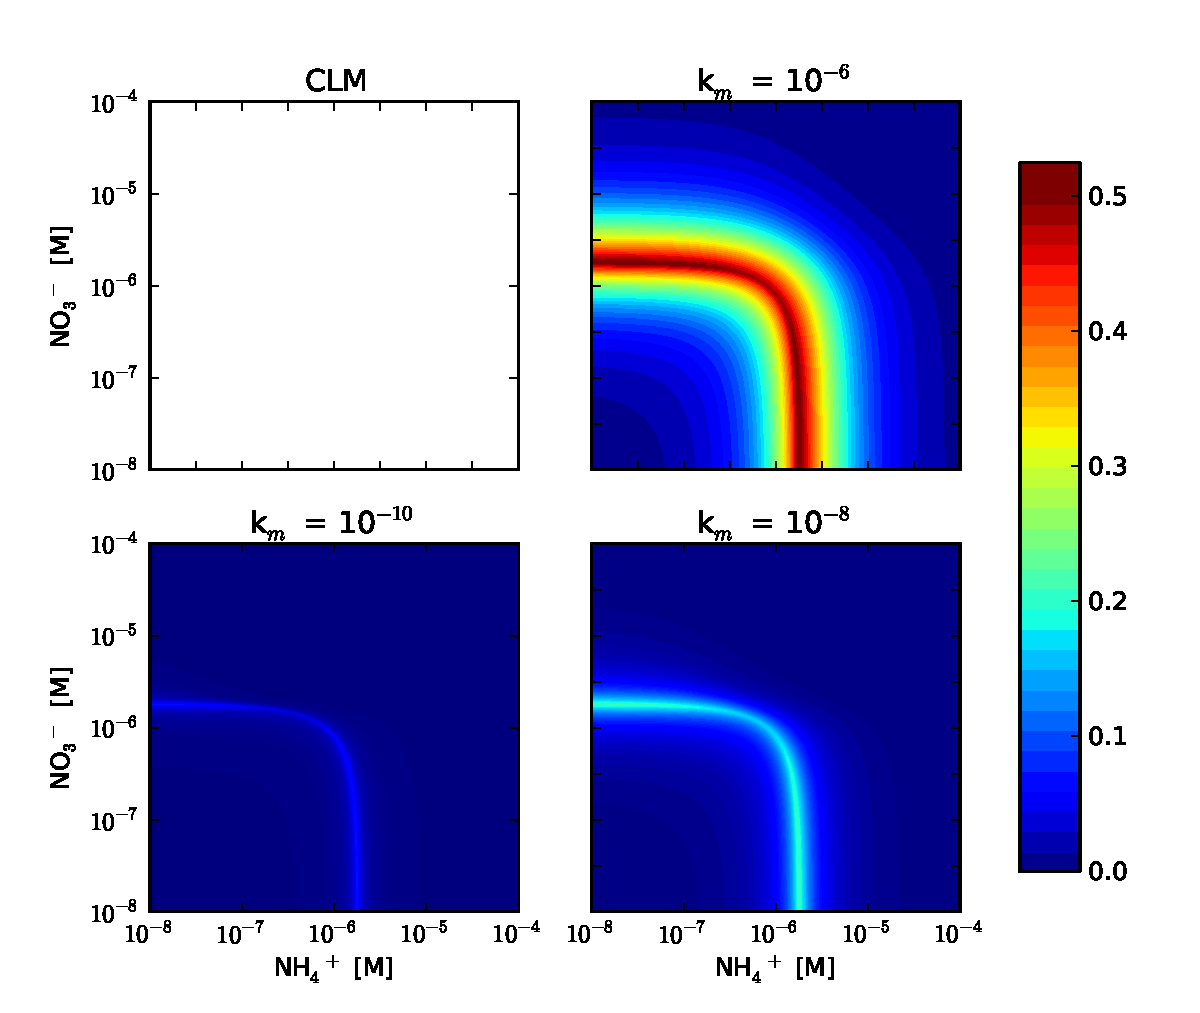
\includegraphics[width=12cm]{../figs/fig06/uptaked.pdf}
%\caption{The difference plots for Fig. (\ref{fig:demanddistribution}).}
%\label{fig:demanddistributiondiff}
%\end{figure}

%\clearpage
\end{document}
